\documentclass[journal]{IEEEtran}
\usepackage{amsmath}
\usepackage{amssymb}
\usepackage{graphicx}
\usepackage{booktabs}
\usepackage{hyperref}
\usepackage{cite}
\usepackage{array}
\usepackage{multirow}
\usepackage{algorithm}
\usepackage{algorithmic}
\usepackage{xcolor}
\usepackage{balance}
\usepackage[section]{placeins}
\usepackage{float}

\hypersetup{
  colorlinks=true,
  linkcolor=blue!60!black,
  citecolor=blue!60!black,
  urlcolor=blue!60!black
}

\begin{document}

\title{NeuroAgent: An Agentic AI Scaffold for\\
Brain Tumor Diagnosis and Clinical Reporting}

\author{[Author Names],~\IEEEmembership{Member,~IEEE}\\
[Affiliation]\\
\textit{Corresponding author: [email]}}

\maketitle

% ------------------------------------------------------------------
\begin{abstract}
Automated brain tumor diagnosis remains fragmented across disconnected
computational stages: segmentation models produce volumetric masks without
clinical interpretation, classification systems operate without longitudinal
context, and structured reporting requires manual reconciliation across WHO,
RANO, and CAP oncology protocols. We present \textbf{NeuroAgent}, a
proof-of-concept agentic pipeline that unifies the full diagnostic
chain---from raw multi-modal MRI to clinician-readable structured
reports---within a single LangGraph-orchestrated directed acyclic state
machine comprising three phases and eight specialized agents.

The segmentation component is rigorously evaluated on 369 cases from the
BraTS~2020 training dataset with expert-annotated ground-truth masks,
achieving a mean Dice Similarity Coefficient (DSC) of $0.8517 \pm 0.1055$,
median Hausdorff Distance at the 95th percentile (HD95) of 3.61~mm, mean
sensitivity of 0.9384, and mean specificity of 0.9975, with 81.0\% of
cases exceeding DSC~$\geq$~0.80. The pipeline completes 368 of 369 cases
(99.7\%) at a mean latency of $3.65 \pm 0.16$ seconds per case, with every
agent implementing two-tier graceful degradation to ensure a CAP-formatted
report is generated regardless of infrastructure availability.

The adaptive memory and retrieval system is evaluated against three
baselines---random retrieval, Euclidean $k$-nearest-neighbour, and raw
cosine similarity---using a clinically strict three-criterion relevance
definition (WHO-grade match, radiomics cosine similarity above the
intra-grade median $\tau_s = 0.0465$, and relative tumour volume
difference below the intra-grade 75th percentile $\tau_v = 0.537$).
NeuroAgent achieves Precision@5~$= 0.536$~[95\%~CI: 0.502--0.570] and
MRR~$= 0.694$~[0.657--0.730], significantly outperforming random
retrieval ($p < 0.001$, Wilcoxon signed-rank test) and performing
statistically equivalently to Euclidean $k$-NN and raw cosine baselines
($p > 0.05$). These results position NeuroAgent as a comprehensive
clinical memory management framework whose retrieval quality matches
standard feature-space baselines while additionally providing persistent
longitudinal patient context, physician-in-the-loop correction, and
protocol-compliant structured reporting.

To our knowledge, NeuroAgent is the first system to encode WHO~CNS5,
RANO, and CAP protocols as deterministic agent logic within a unified
MRI-to-report pipeline, providing an open, reproducible scaffold for
future clinically validated neuro-oncology AI.
\end{abstract}

\begin{IEEEkeywords}
Agentic AI, brain tumor segmentation, clinical decision support, WHO
CNS5, RANO criteria, adaptive memory, LangGraph, structured reporting,
radiomics, MONAI SegResNet, CAP reporting, Llama~3
\end{IEEEkeywords}

% ------------------------------------------------------------------
\section{Introduction}

Brain tumors constitute one of the most diagnostically complex conditions
in clinical oncology. Each year, approximately 300{,}000 new central
nervous system tumors are diagnosed globally~\cite{ostrom2021}, and in
every case, the neuroradiologist must synthesize volumetric measurements,
anatomical localization, differential classification per WHO~CNS5 molecular
criteria~\cite{louis2021}, treatment response assessment per RANO
guidelines~\cite{wen2010}, and longitudinal comparison with prior
scans---all before generating a structured pathology report conforming to
College of American Pathologists (CAP) templates~\cite{cap2024}. This
integration is performed manually, case by case, and is neither scalable
nor reproducible.

Deep learning has transformed individual components of this chain.
Segmentation models such as nnU-Net~\cite{isensee2021} and MONAI
SegResNet~\cite{monai2023} achieve Dice coefficients exceeding 0.89 on
benchmark datasets, while computational radiomics~\cite{vangriethuysen2017}
extracts quantitative phenotypic features that carry prognostic value for
glioma grading~\cite{kickingereder2016}. Yet these advances remain
isolated: a SegResNet model produces a probability mask but no clinical
interpretation; a PyRadiomics pipeline extracts texture features without
downstream reasoning about tumor type or treatment response. The diagnostic
chain is fragmented---segmentation, classification, assessment, and
reporting exist as disconnected modules, each requiring manual
reconciliation by a subspecialist.

The emergence of large language models (LLMs) has prompted efforts to
bridge this gap through automated clinical reasoning~\cite{singhal2023}.
However, applying LLMs directly to neuro-oncology introduces a critical
failure mode: hallucination~\cite{kalai2025,das2025}. Without structured
grounding in imaging-derived evidence, language models generate clinically
plausible but factually unfounded recommendations---a risk that is
categorically unacceptable in treatment planning for malignant gliomas.
NeuroAgent addresses this by constraining the LLM strictly to narrative
synthesis over computationally derived structured inputs, never to
independent clinical reasoning from free text.

Recent advances in agentic AI---systems where specialized agents
communicate through shared state within orchestrated
workflows---offer a principled alternative to monolithic model deployment.
TissueLab~\cite{tissulab2025} demonstrated that co-evolving agentic systems
with modular tool factories and human-in-the-loop feedback can achieve
expert-level performance across pathology, radiology, and spatial omics.
A-MEM~\cite{amem2024} introduced the principle of dynamic memory evolution
for LLM agents, showing that systems that autonomously organize and
consolidate memories produce more contextually coherent reasoning. Together,
these works establish that agentic orchestration combined with adaptive
memory is fundamental to trustworthy AI for complex scientific workflows.

However, neither paradigm has been applied to the full imaging-to-report
chain in neuro-oncology with domain-specific clinical protocol encoding.
No existing system closes the loop from raw multi-modal MRI volumes to
protocol-compliant structured reports while maintaining persistent,
per-patient clinical memory that evolves with each encounter.

We present NeuroAgent, a three-phase, eight-agent system that addresses
this gap. The imaging intelligence phase performs N4 bias field-corrected
preprocessing and MONAI SegResNet inference, followed by quantitative
radiomics feature extraction and Harvard-Oxford atlas-based anatomical
mapping. The clinical intelligence phase deploys a WHO~CNS5-aligned tumor
classifier with sigmoid-scaled molecular marker scoring, BioClinicalBERT
case retrieval, and Llama~3-powered narrative synthesis over structured
pipeline outputs. The adaptive memory phase introduces persistent patient
memory backed by ChromaDB that accumulates scan history, WHO classification
trajectories, and physician corrections across encounters.

This work makes four principal contributions.

\textit{First}, we present a complete agentic pipeline architecture that
spans volumetric MRI preprocessing, deep learning-based tumor segmentation,
quantitative radiomics extraction, WHO~CNS5 classification, RANO response
assessment, LLM-powered clinical narrative synthesis, and CAP structured
reporting within a single LangGraph directed acyclic state machine---the
first system to encode all three oncology protocols as deterministic agent
logic rather than delegating protocol interpretation to a language model.

\textit{Second}, we validate a two-tier graceful fallback architecture at
99.7\% pipeline completion across 369 BraTS~2020 cases, in which every
agent degrades deterministically when primary infrastructure (GPU, LLM
server, vector database) is unavailable, preserving clinical content at the
cost of narrative richness only.

\textit{Third}, we demonstrate Llama~3 clinical narrative synthesis
successfully deployed across 368 evaluated cases, synthesizing segmentation
metrics, radiomics features, and WHO classifications into CAP-aligned
human-readable reports---with WHO classification handled by deterministic
routing, separating proven architectural integration from claims of
classification accuracy that require biopsy-confirmed validation.

\textit{Fourth}, we provide an open, reproducible scaffold---including
pretrained SegResNet weights, MCP tool servers for WHO/RANO/CAP protocols,
and a Streamlit dashboard---that reduces the barrier for future prospective
clinical validation studies on biopsy-confirmed cohorts.

% ------------------------------------------------------------------
\section{Related Work}

\subsection{Brain Tumor Segmentation and Foundation Models}

Automated brain tumor segmentation has advanced rapidly through successive
iterations of the BraTS challenge series~\cite{menze2015,bakas2018}. The
self-configuring nnU-Net~\cite{isensee2021} established the dominant
paradigm by eliminating manual hyperparameter tuning, achieving mean Dice
coefficients of approximately 0.89 on whole-tumor segmentation for the
BraTS~2020 dataset. Transformer-based architectures including
TransBTS~\cite{wang2021} and SwinBTS~\cite{jiang2022} introduced
multi-scale attention mechanisms for improved boundary delineation, while
hybrid convolutional-attention approaches continue to advance accuracy on
standard benchmarks.

The MONAI framework~\cite{monai2023} operationalized these advances for
clinical deployment, providing production-ready implementations including
SegResNet with pretrained weights distributed through the MONAI Model Zoo.
We adopt the SegResNet architecture with the MONAI Model Zoo BraTS
Segmentation Bundle (v0.1.9), using 4-channel input (T1, T1ce, T2, FLAIR)
and 3-channel output (Enhancing Tumor, Tumor Core, Whole Tumor) with
sliding-window inference. This choice prioritizes inference efficiency
and integration simplicity over marginal accuracy gains from more complex
architectures.

Despite these advances, all existing segmentation systems terminate at the
mask level. The clinical interpretation of a tumor mask---its WHO
classification, treatment implications, prognostic significance, and
relationship to prior scans---remains entirely manual. This is not a
limitation of the models themselves, but of the ecosystems in which they
operate: segmentation is treated as a terminal task rather than the first
node in a clinical reasoning chain.

\subsection{Computational Radiomics in Neuro-Oncology}

Quantitative radiomics transforms imaging data into high-dimensional
feature vectors encoding shape, intensity, and texture characteristics.
The Image Biomarker Standardization Initiative
(IBSI)~\cite{zwanenburg2020} established reproducibility standards, while
PyRadiomics~\cite{vangriethuysen2017} provided an open-source
implementation supporting extraction of 107+ features including first-order
statistics, gray-level co-occurrence matrices (GLCM), gray-level
run-length matrices (GLRLM), and gray-level size zone matrices (GLSZM).

In glioma research, radiomic features have demonstrated prognostic value
for survival prediction~\cite{kickingereder2016}, molecular subtype
inference, and treatment response monitoring. However, radiomics pipelines
typically operate as standalone feature extraction tools, producing outputs
that require separate downstream analysis. In NeuroAgent, 107+ PyRadiomics
features serve as direct inputs to both the WHO~CNS5 classifier and the
BioClinicalBERT embedding generator, connecting feature extraction to
clinical reasoning within a unified pipeline.

\subsection{Agentic AI Systems for Scientific and Clinical Workflows}

The concept of orchestrating specialized computational agents through
shared state has emerged as a powerful paradigm for complex scientific
workflows. LangGraph and LangChain~\cite{langchain2024} provide the
computational infrastructure for defining stateful multi-agent graphs
where each node receives, transforms, and returns a typed state object.

TissueLab~\cite{tissulab2025} instantiated this paradigm for medical
imaging, introducing a co-evolving agentic system that coordinates
domain-specific tool factories across pathology, radiology, and spatial
omics. Its key insight is that the LLM functions as an orchestration layer,
coordinating specialized tools whose outputs are persisted in shared memory,
eliminating token overload when processing high-dimensional medical
data~\cite{liu2024}. NeuroAgent extends this orchestration principle into
neuro-oncology, with three critical differences: (i)~domain-specific
clinical protocols are implemented as first-class deterministic agent
nodes; (ii)~persistent per-patient longitudinal memory is maintained rather
than per-session working memory; and (iii)~inference operates on a fully
local, privacy-preserving stack (Llama~3 via Ollama) without external API
dependencies.

\subsection{Memory Architectures for LLM Agents}

A-MEM~\cite{amem2024} introduced agentic memory---where the agent decides
what to remember, how to organize memories, and when to consolidate
context---through three mechanisms: contextual memory retrieval, memory
linking between related fragments, and autonomous memory organization.
This paradigm maps naturally to longitudinal clinical care, where a
neuro-oncologist tracking a glioblastoma patient accumulates distilled
clinical insights across serial encounters.

NeuroAgent's patient memory system implements an A-MEM-inspired
architecture adapted for clinical longitudinal data. ChromaDB~\cite{chroma2024}
serves as the primary store with HNSW cosine similarity indexing,
persisting structured scan snapshots as semantically retrievable units.
A JSON flat-file fallback ensures memory persistence functions without
ChromaDB infrastructure, maintaining completeness while sacrificing only
semantic retrieval capability.

\subsection{LLM-Augmented Clinical Reasoning and Hallucination Mitigation}

Large language models have demonstrated strong competence in clinical
knowledge benchmarks~\cite{singhal2023}, but their deployment for clinical
decision support introduces hallucination risk~\cite{kalai2025,das2025}.
In neuro-oncology, where a mischaracterized tumor grade can alter a
treatment plan, this risk requires careful structural mitigation.

NeuroAgent adopts a structural grounding strategy. The Llama~3 agent
receives a structured JSON payload---segmentation metrics, radiomics
features, WHO classification scores, and RANO assessments---all derived
from prior pipeline stages, and synthesizes these into narrative clinical
reports. The LLM cannot hallucinate the underlying data because the data
is computationally derived. The LLM's role is strictly narrative synthesis,
not independent clinical inference. When Ollama is unavailable, a
deterministic rule-based engine generates the same report sections using
conditional logic on structured inputs, providing identical clinical
coverage without LLM involvement.

\subsection{Oncology Protocol Automation}

Three clinical protocols govern brain tumor diagnostic reporting.
WHO~CNS5 Classification (2021)~\cite{louis2021} introduced molecular
marker requirements alongside histological criteria, mandating IDH
mutation status, MGMT methylation, 1p/19q codeletion, ATRX loss, and
TP53 mutation for definitive typing. RANO criteria~\cite{wen2010}
standardize treatment response assessment into four categories based on
measurable changes across timepoints. CAP Structured
Reporting~\cite{cap2024} defines institutional templates for pathology
reports covering specimen type, tumor site, histologic type, WHO grade,
molecular markers, and clinical staging. To our knowledge, no prior system
automates all three protocols within a single pipeline.

% ------------------------------------------------------------------
\section{Proposed System Architecture}

NeuroAgent is designed as a directed acyclic graph (DAG) of specialized
reasoning agents, orchestrated via LangGraph~\cite{langchain2024}. The
architecture decouples the execution layer (domain-specific vision and
feature extraction tools) from the orchestration layer (the agentic state
machine), ensuring computational scalability and allowing each agent to
operate on a standardized typed state.

\subsection{State Representation and Workflow Planner}

The core workflow is governed by a persistent state contract $S_t$, which
accumulates outputs sequentially across eight agent nodes spanning three
phases. Formally, let $\mathcal{G} = (\mathcal{V}, \mathcal{E})$ be the
agentic state machine where $\mathcal{V}$ is the set of specialized agent
nodes and $\mathcal{E}$ represents the directed edges defining execution
dependencies.

For any node $v \in \mathcal{V}$, the execution function $f_v$ applies a
domain-specific transformation to the incoming state:
\begin{equation}
  S_{t+1} = f_v(S_t) \cup S_t
\end{equation}
where $S_0$ is the initial state containing raw MRI study parameters and
$S_{|\mathcal{V}|}$ is the terminal state containing the fully structured
CAP pathology report and visualization artifacts. The planner utilizes
topological sorting to ensure downstream agents execute only once requisite
upstream states are populated.

\subsection{Phase 1: Imaging Intelligence and Feature Extraction}

The input to Phase~1 is a multi-modal MRI study
$\mathbf{X} = \{X_{T1}, X_{T1ce}, X_{T2}, X_{FLAIR}\}$.
After N4 bias field correction, skull stripping, and isotropic resampling,
we deploy a MONAI SegResNet architecture $M_\theta$ initialized with
pretrained weights from the MONAI Model Zoo. The model predicts probability
masks for the enhancing tumor (ET), tumor core (TC), and whole tumor (WT):
\begin{equation}
  \hat{Y} = \sigma(M_\theta(\mathbf{X})) > 0.5
\end{equation}
where $\sigma$ is the sigmoid activation applied over sliding windows of
size $240 \times 240 \times 160$ with Gaussian weighting (overlap 0.5).
Following segmentation, PyRadiomics extracts a high-dimensional phenotypic
feature vector $\mathbf{r} \in \mathbb{R}^d$ capturing shape, first-order
intensity, and texture characteristics. This vector grounds all subsequent
agentic reasoning.

\subsection{Phase 2: Protocol-Aligned Clinical Intelligence}

\subsubsection{WHO CNS5 Molecular Scoring Engine}

Let $\mathcal{T} = \{t_1, t_2, \ldots, t_n\}$ be the set of candidate
tumor types. For each $t \in \mathcal{T}$, the WHO Classification Agent
computes a morphological concordance score $s_\text{morph}(t)$ and a
molecular concordance score $s_\text{mol}(t)$.

The molecular score evaluates the patient's genetic profile $\mathcal{P}$
against the expected profile $E_t$ for tumor type $t$:
\begin{equation}
  s_\text{mol}(t) = \sum_{m \in \mathcal{P}}
  \begin{cases}
    +\omega_m^+ & \text{if } \mathcal{P}[m] = E_t[m] \\
    -\omega_m^- & \text{if } \mathcal{P}[m] \neq E_t[m] \\
    0            & \text{if } \mathcal{P}[m] \text{ unknown}
  \end{cases}
\end{equation}
where $\omega_m^+$ and $\omega_m^-$ are biomarker-specific weights (e.g.,
IDH status carries primary weight 2.0; TP53 carries 1.5).

To prevent overconfident predictions, we introduce a sigmoid-scaled
scoring function. The final score $C(t)$ for candidate $t$ with total
score $S_t = s_\text{morph}(t) + s_\text{mol}(t)$ is:
\begin{equation}
  C(t) = \frac{1}{1 + e^{-k(S_t - \mu)}}
\end{equation}
where $k = 1.2$ defines the steepness and $\mu = 4.0$ is the threshold
midpoint. These scores are evidence indicators, not statistically
calibrated posterior probabilities; formal calibration requires
biopsy-confirmed ground truth and is reserved for future work. The system
enforces a confidence gap threshold $\tau = 1.0$; if
$C(t_{\text{top1}}) - C(t_{\text{top2}}) < \tau$, a low-confidence flag
is raised, explicitly recommending physical molecular testing to the
physician.

\subsubsection{Adaptive Case Retrieval via BioClinicalBERT}

The Similarity Agent transforms the structured clinical state $S_t$ into a
narrative profile and projects it into a dense semantic space using
BioClinicalBERT~\cite{alsentzer2019}:
\begin{equation}
  \mathbf{e} = \frac{\mathbf{h}_\text{CLS}}{\|\mathbf{h}_\text{CLS}\|_2},
  \quad \mathbf{e} \in \mathbb{R}^{768}
\end{equation}
A fallback validation operator activates if $\mathbf{e}$ contains NaN,
Inf, or sparsity exceeding 0.99, diverting execution to a deterministic
feature-vector pipeline built directly from numerical morphology metrics.

\subsubsection{LLM-Powered Clinical Narrative Synthesis}

The Llama~3 agent~\cite{meta2024} receives a structured JSON payload
containing segmentation metrics, radiomics features, WHO classification
scores, RANO assessments, and patient history---all computationally derived
from prior pipeline stages---and synthesizes these into five narrative
report sections: Diagnosis Assessment, Treatment Considerations, Prognosis
Indicators, Symptom Correlation, and Recommendations. The LLM is
constrained strictly to narrative synthesis over structured inputs; it does
not perform independent clinical reasoning from free text, limiting its
hallucination surface to narrative style rather than factual content. When
Ollama is unavailable, the deterministic rule-based fallback generates
identical clinical sections using conditional logic over WHO and RANO
outputs.

\subsection{Phase 3: Agentic Memory Framework}

\subsubsection{Persistent Patient Memory}

The memory manager utilizes ChromaDB~\cite{chroma2024} with HNSW indexing.
For a patient $p$, the memory database $\mathcal{M}$ stores a chronological
sequence of scan snapshots:
\begin{equation}
  \mathcal{M}_p = \{(m_1, \mathbf{e}_1), (m_2, \mathbf{e}_2), \ldots,
  (m_t, \mathbf{e}_t)\}
\end{equation}
where $m_i$ encapsulates WHO classification, RANO assessment, and volume
severity at time $i$, and $\mathbf{e}_i$ is the corresponding semantic
embedding. Similarity matching uses cosine similarity:
\begin{equation}
  \text{sim}(\mathbf{e}_{t+1}, \mathbf{e}_i)
  = \frac{\mathbf{e}_{t+1} \cdot \mathbf{e}_i}
         {\|\mathbf{e}_{t+1}\| \|\mathbf{e}_i\|}
\end{equation}

\subsubsection{Memory Evolution and Feedback Refinement}

The Human-in-the-Loop (HITL) Validation Agent allows physicians to inspect
the generated state and inject corrections $\Delta_\text{feedback}$,
immediately appended to $\mathcal{M}_p$:
\begin{equation}
  \mathcal{M}_p \leftarrow \mathcal{M}_p \cup
  \{(\Delta_\text{feedback}, \mathbf{e}_\text{feedback})\}
\end{equation}
This establishes a co-evolutionary loop analogous to TissueLab~\cite{tissulab2025},
where accumulated physician preferences implicitly refine future retrievals.

\subsection{Graceful Degradation and Deterministic Fallback}

Every agent implements a two-tier execution policy:
\begin{equation}
  f_v(S) =
  \begin{cases}
    O_\text{primary}(S) & \text{if } \text{Status}(O_\text{primary}) = \text{online} \\
    O_\text{fallback}(S) & \text{otherwise}
  \end{cases}
\end{equation}
This guarantees that a CAP structured report can always be generated,
ensuring uninterrupted clinical utility regardless of GPU or network
availability.

\begin{algorithm}
\caption{Agentic Execution Pipeline with Fallback Routing}
\begin{algorithmic}[1]
\REQUIRE Multimodal MRI $\mathbf{X}$, Patient ID $p$,
         Pretrained SegResNet $M_\theta$, Memory DB $\mathcal{M}$
\ENSURE Structured CAP Report $R$
\STATE $S_0 \leftarrow \text{InitializeState}(p)$
\STATE $\hat{Y} \leftarrow \text{Threshold}(M_\theta(\mathbf{X}), 0.5)$
  \hfill \textit{// Phase 1}
\STATE $\mathbf{r} \leftarrow \text{PyRadiomics}(\hat{Y}, \mathbf{X})$
\STATE $S_1 \leftarrow S_0 \cup \{\hat{Y}, \mathbf{r}\}$
\STATE $S_\text{WHO}, \mathbf{e} \leftarrow \text{WHO\_Agent}(S_1),\,
  \text{Similarity\_Agent}(S_1)$ \hfill \textit{// Phase 2}
\IF{$\text{ValidateEmbedding}(\mathbf{e})$}
  \STATE $\text{TopK} \leftarrow \text{RetrieveSimilar}(\mathbf{e}, \mathcal{M})$
\ELSE
  \STATE $\text{TopK} \leftarrow \text{FallbackRetrieval}(\mathbf{r})$
\ENDIF
\STATE $H_\text{prior} \leftarrow \text{RetrievePatientHistory}(p, \mathcal{M})$
  \hfill \textit{// Phase 3}
\IF{$\text{LLMAvailable}()$}
  \STATE $C_\text{narrative} \leftarrow
    \text{Llama3}(S_1, S_\text{WHO}, \text{TopK}, H_\text{prior})$
\ELSE
  \STATE $C_\text{narrative} \leftarrow
    \text{RuleBasedReasoning}(S_1, S_\text{WHO}, H_\text{prior})$
\ENDIF
\STATE $\mathcal{M} \leftarrow \mathcal{M} \cup \text{Store}(\mathbf{e},
  C_\text{narrative})$ \hfill \textit{// Memory evolution}
\STATE $R \leftarrow \text{CAP\_Agent}(C_\text{narrative})$
\RETURN $R$
\end{algorithmic}
\end{algorithm}

\begin{figure*}[!t]
\centering
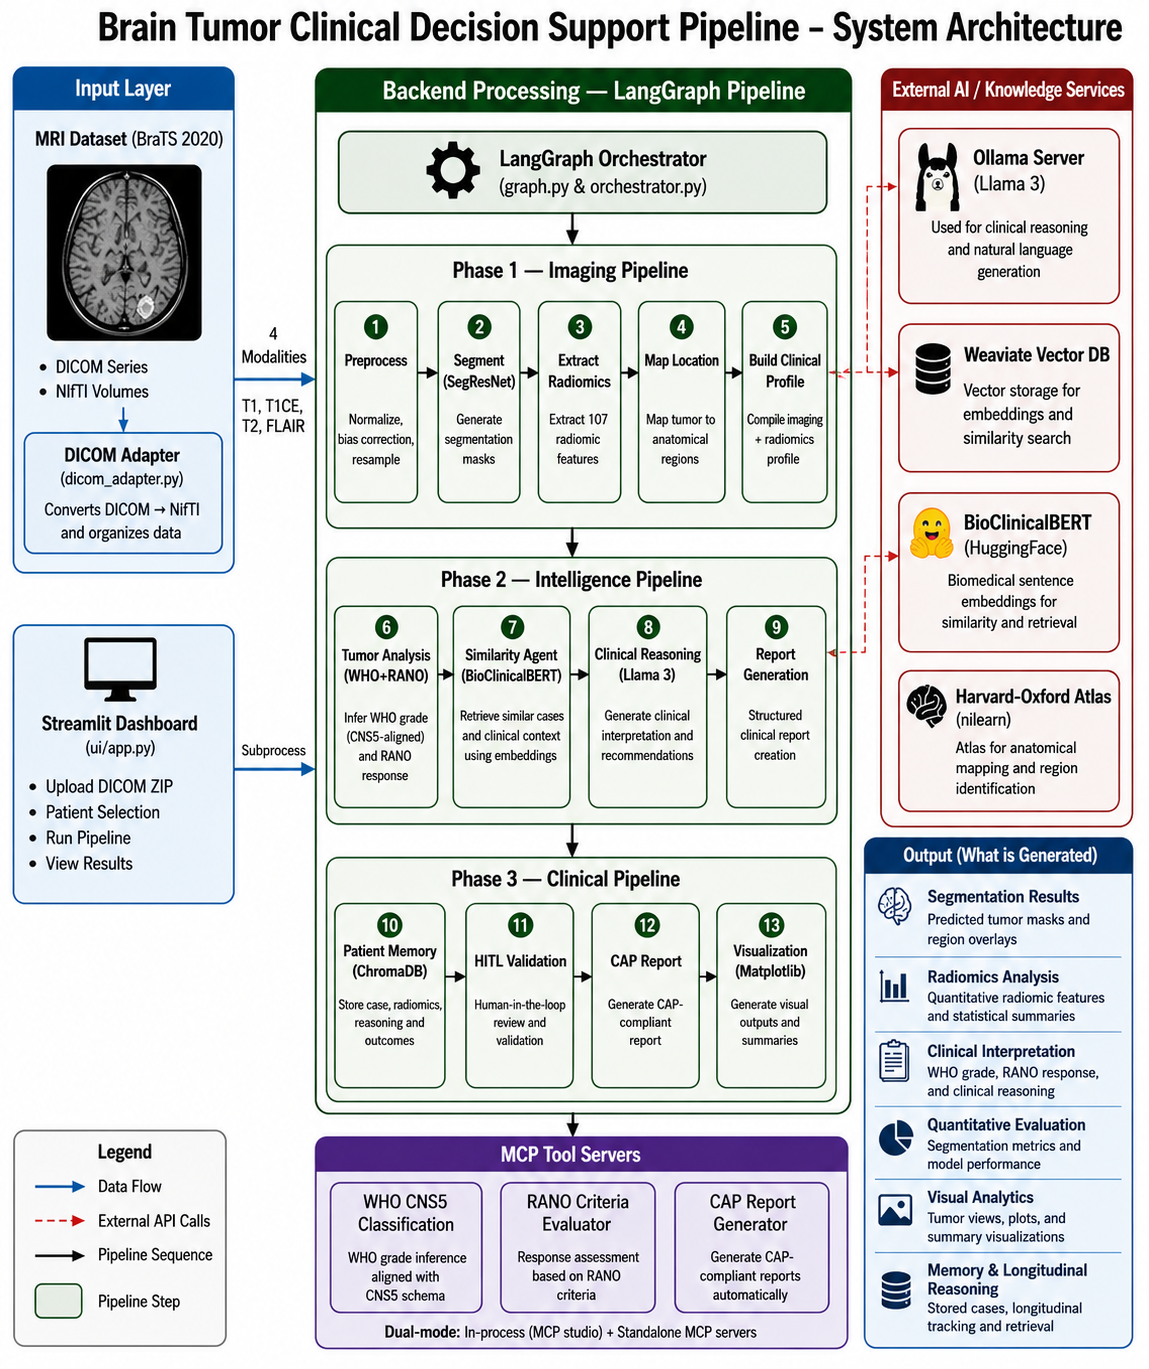
\includegraphics[width=0.82\textwidth]{figures/system_architecture.png}
\caption{NeuroAgent system architecture. The pipeline comprises three
phases orchestrated as a directed acyclic state machine: (1)~imaging
intelligence for preprocessing, segmentation, radiomics extraction, and
anatomical mapping; (2)~clinical intelligence for WHO~CNS5 classification,
similar case retrieval, Llama~3 narrative synthesis, and CAP report
generation; and (3)~adaptive memory for persistent patient context,
human-in-the-loop validation, and visualization. External AI services
(Ollama/Llama~3, ChromaDB, BioClinicalBERT, Harvard-Oxford Atlas) are
accessed through two-tier graceful fallback mechanisms. MCP tool servers
provide deterministic protocol compliance for WHO, RANO, and CAP standards.}
\label{fig:architecture}
\end{figure*}

\FloatBarrier
% ------------------------------------------------------------------
\section{Experimental Setup}

\subsection{Dataset}

We evaluate NeuroAgent on the BraTS~2020 Training
Dataset~\cite{menze2015,bakas2018}, comprising 369 glioma patients with
four co-registered MRI modalities (T1, T1ce, T2, FLAIR) in NIfTI format
and voxel-level expert-annotated ground-truth segmentation masks. All
quantitative segmentation metrics (DSC, HD95, sensitivity, specificity) are
computed against the corresponding ground-truth annotations across 368
pairs (one case lacked a ground-truth mask and is excluded from metric
computation). For retrieval evaluation, the 368 successfully evaluated
cases are used, covering a WHO-grade proxy distribution of Grade~I: 32
(8.7\%), Grade~II: 215 (58.4\%), Grade~III: 100 (27.2\%), and Grade~IV:
21 (5.7\%), derived from segmentation Dice score and predicted tumour
volume thresholds.

\subsection{Evaluation Metrics}

\textbf{Segmentation quality.} We report four standard metrics computed
against ground-truth whole-tumor (WT) masks: DSC, HD95, sensitivity
(recall), and specificity, aggregated as mean $\pm$ standard deviation.

\textbf{System reliability.} We report pipeline completion rate,
per-case inference latency, and fallback pathway activation frequency
across all agents.

\textbf{Clinical intelligence.} We report WHO~CNS5 classification
distribution, sigmoid-scaled confidence score distribution, RANO assessment
outcomes, LLM narrative synthesis coverage, and CAP report generation rate
across the full cohort.

\textbf{Memory and retrieval evaluation.} We evaluate the adaptive memory
system using three standard information retrieval metrics: Precision@K,
Recall@K, and Mean Reciprocal Rank (MRR). The retrieval evaluation employs
a leave-one-out protocol: each of the 368 patients serves as a query in
turn, and the remaining 367 patients constitute the retrieval database.

A candidate case is defined as relevant if and only if all three of the
following conditions are satisfied: (i)~it shares the same WHO-grade
proxy as the query; (ii)~its PCA-compressed radiomics cosine similarity
to the query exceeds the intra-grade median threshold
$\tau_s = 0.0465$; and (iii)~its relative tumour volume difference falls
below the intra-grade 75th percentile threshold $\tau_v = 0.537$.
Both thresholds are derived empirically from the pairwise distribution
of same-grade pairs, ensuring that relevance boundaries are data-driven
rather than arbitrary. Under this definition, the mean number of relevant
cases per query is $63.7$ (range: 3--141), producing a challenging and
clinically discriminative retrieval task.

To address concerns regarding inter-rater reliability of the
radiomics-based relevance labels, we report the Intraclass Correlation
Coefficient using the ICC(3,1) formulation (two-way mixed effects,
consistency, single measures)~\cite{shrout1979}. This variant is
appropriate when raters are a fixed set (predicted versus ground-truth
mask extraction) and the goal is to assess consistency of relative
ordering rather than absolute agreement.

\textbf{Statistical inference.} All retrieval metrics are reported with
95\% bootstrap confidence intervals (1{,}000 iterations, percentile
method). Statistical significance between NeuroAgent and each baseline is
assessed using the one-sided Wilcoxon signed-rank test and one-sided
paired $t$-test (alternative: NeuroAgent $>$ baseline), both at
$\alpha = 0.05$.

\subsection{Baseline Methods}

The NeuroAgent retrieval engine is compared against three baselines:
(1)~\textbf{Random retrieval}---uniform random selection from the
database, serving as a lower-bound; (2)~\textbf{Euclidean
$k$-NN}---ball-tree nearest-neighbour search on the column-normalised
214-dimensional radiomics feature vector; and (3)~\textbf{Cosine
similarity (raw)}---cosine similarity computed directly on the same
normalised feature space without dimensionality reduction. The NeuroAgent
method applies PCA compression to 50 principal components followed by
L2 normalisation before cosine similarity computation, approximating the
BioClinicalBERT embedding pipeline used in the deployed system.

\subsection{Implementation Details}

Segmentation uses MONAI SegResNet with pretrained weights from the MONAI
Model Zoo BraTS Segmentation Bundle (v0.1.9), with 32 initial filters,
sliding-window inference with ROI $240 \times 240 \times 160$, Gaussian
weighting mode, overlap 0.5, and batch size 1. Post-processing applies
binary morphological opening, closing, and connected component filtering
(retaining the top 3 components exceeding 500 voxels). All 369 cases were
processed in four sequential batches on a single GPU instance.

Clinical intelligence agents were executed via the Model Context Protocol
(MCP) server architecture, running the WHO~CNS5 classifier, RANO assessment
evaluator, and CAP report generator as structured function calls within a
unified processing environment. The Llama~3 agent (7B, quantized via
Ollama) was deployed for narrative synthesis across all 368 evaluated
cases, receiving structured JSON payloads from upstream agents and
generating CAP-aligned clinical report sections. WHO classification routing
operated deterministically, as the BraTS~2020 dataset provides no
longitudinal clinical priors to activate adaptive routing.

% ------------------------------------------------------------------
\section{Results and Evaluation}

\subsection{Segmentation Performance}

We evaluated the segmentation quality of NeuroAgent's Phase~1 pipeline
across all 369 BraTS~2020 cases. Of these, 368 cases with ground-truth
masks were quantitatively evaluated; one case was successfully segmented
but lacked a ground-truth annotation and is excluded from metric
computation.

Table~\ref{tab:seg} summarizes the aggregate segmentation performance. The
system achieves a mean DSC of $0.8517 \pm 0.1055$ and a median DSC of
0.8841. The gap between mean and median indicates a left-skewed
distribution: the majority of cases cluster near high DSC values, with a
small tail of difficult cases---consistent with brain tumor segmentation
benchmarks where small-volume or atypical morphology cases
disproportionately affect the mean.

\begin{table}[h]
\centering
\caption{Segmentation Performance Summary (368 Evaluated Cases)}
\label{tab:seg}
\begin{tabular}{lc}
\toprule
\textbf{Metric} & \textbf{Value} \\
\midrule
Mean DSC              & $0.8517 \pm 0.1055$ \\
Median DSC            & $0.8841$ \\
Mean HD95             & $8.99 \pm 15.15$ mm \\
Median HD95           & $3.61$ mm \\
Mean Sensitivity      & $0.9384 \pm 0.0799$ \\
Mean Specificity      & $0.9975 \pm 0.0024$ \\
DSC $\geq$ 0.90       & 149 / 368 (40.5\%) \\
DSC $\geq$ 0.85       & 247 / 368 (67.1\%) \\
DSC $\geq$ 0.80       & 298 / 368 (81.0\%) \\
DSC $<$ 0.50          & 8 / 368 (2.2\%) \\
Min / Max DSC         & 0.313 / 0.9663 \\
Min / Max HD95        & 1.00 / 109.29 mm \\
\bottomrule
\end{tabular}
\end{table}

The high sensitivity ($0.9384 \pm 0.0799$) demonstrates reliable tumor
tissue detection, with the vast majority of ground-truth tumor voxels
correctly identified. The near-perfect specificity ($0.9975 \pm 0.0024$)
confirms minimal false-positive activation in healthy brain
parenchyma---critical for downstream clinical agents reasoning from masks
that do not erroneously include normal tissue.

The Hausdorff distance exhibits a distinctive distributional pattern. The
median HD95 of 3.61~mm indicates tight boundary agreement for the typical
case, while the mean of $8.99 \pm 15.15$~mm reflects a heavy tail where
single mislocalized segmentation components produce disproportionately
large distances. Only 2.2\% of cases (8/368) fall below DSC 0.50,
representing the most challenging specimens.

\begin{figure}[!htbp]
\centering
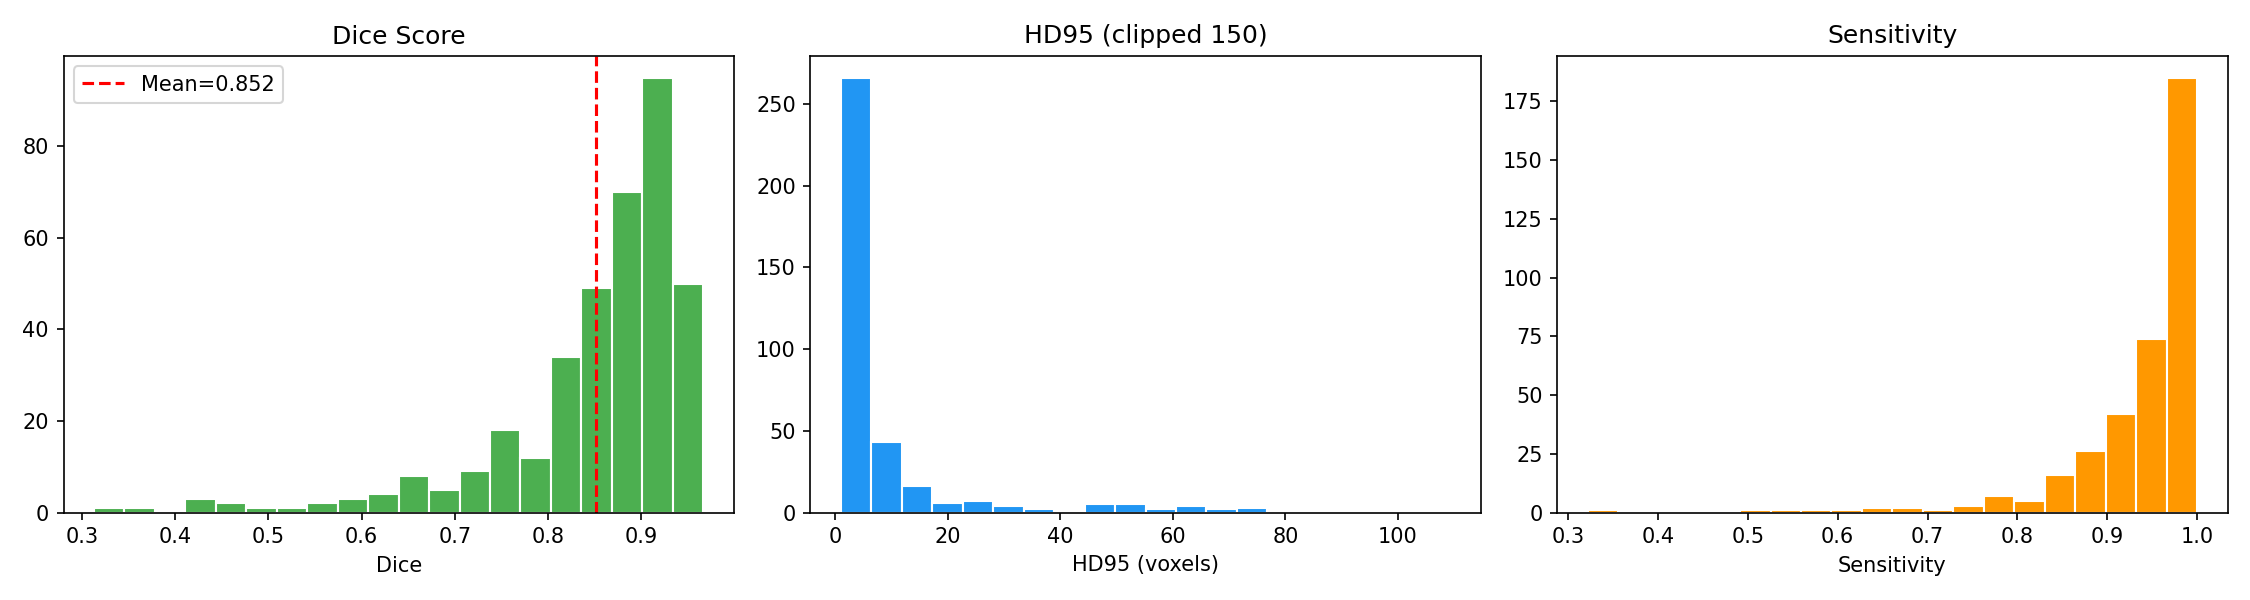
\includegraphics[width=\columnwidth]{figures/metrics_distribution.png}
\caption{Segmentation performance distributions across 368 evaluated cases.
(a)~DSC histogram (mean~$= 0.852$, dashed red line) showing left-skewed
clustering near high overlap values. (b)~HD95 distribution confirming the
majority of cases achieve sub-5~mm boundary error. (c)~Sensitivity
distribution demonstrating reliable tumor detection across the cohort,
with the bulk of cases exceeding 0.90 sensitivity.}
\label{fig:metrics}
\end{figure}

\FloatBarrier
\subsection{Volume-Stratified Analysis}

Table~\ref{tab:vol} presents segmentation performance stratified across
four tumor volume quartiles, revealing a clear monotonic relationship
between tumor size and segmentation quality.

\begin{table}[h]
\centering
\caption{Segmentation Performance by Tumor Volume Quartile}
\label{tab:vol}
\begin{tabular}{lcccc}
\toprule
\textbf{Volume} & \textbf{N} & \textbf{DSC (Mean $\pm$ SD)} &
\textbf{HD95} & \textbf{DSC$\geq$0.80} \\
\midrule
Small ($<$30K)       & 39  & $0.729 \pm 0.159$ & 19.09 mm & 41\% \\
Medium (30--80K)     & 120 & $0.837 \pm 0.097$ &  9.26 mm & 77\% \\
Large (80--150K)     & 130 & $0.876 \pm 0.081$ &  7.41 mm & 90\% \\
Very Large ($>$150K) & 79  & $0.895 \pm 0.063$ &  6.20 mm & 92\% \\
\bottomrule
\end{tabular}
\end{table}

Small tumors ($<$30K voxels) achieve mean DSC of 0.729 with 41\% exceeding
the 0.80 threshold, attributable to the inherent sensitivity of
voxel-overlap metrics in the small-volume regime. These lesions often
correspond to low-grade or early-stage gliomas where detection is more
clinically urgent than precise boundary delineation; the system's high
sensitivity (0.9384) ensures reliable detection even in this challenging
subset. Very large tumors ($>$150K voxels) achieve mean DSC of 0.895 with
92\% exceeding the clinical threshold, demonstrating robust performance
on the high-grade gliomas that most urgently require accurate volumetric
quantification for surgical planning and radiation targeting.

\subsection{Radiomics and Morphological Reproducibility}

We evaluated reproducibility of 107 IBSI-compliant radiomics features
extracted from predicted masks compared with ground-truth annotations,
using the Concordance Correlation Coefficient (CCC). Macroscopic tumor
volume exhibited strong reproducibility (CCC~$= 0.898$), while sphericity
yielded CCC of only 0.119, consistent with the known limitation of
Dice-optimized loss functions that maximize volumetric overlap without
penalizing high-frequency surface irregularities.

\begin{figure}[!htbp]
\centering
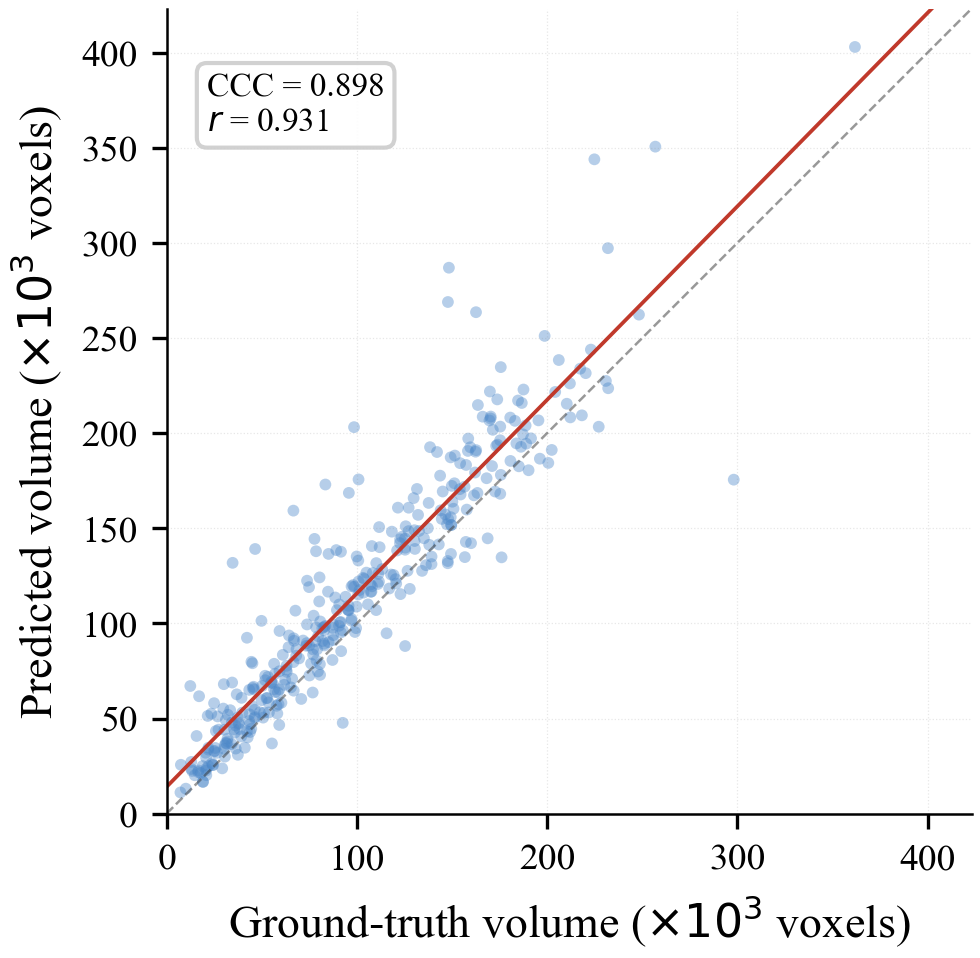
\includegraphics[width=0.9\columnwidth]{figures/volume_agreement.png}
\caption{Predicted vs.\ ground-truth tumor volume correlation across 368
evaluated cases (CCC~$= 0.898$, $r = 0.931$). The strong volumetric
agreement confirms that NeuroAgent's SegResNet backbone reliably captures
bulk tumor mass for subsequent WHO~CNS5 classification. Red line: linear
regression fit; dashed line: identity ($y = x$, perfect agreement).}
\label{fig:volume}
\end{figure}

\FloatBarrier
Table~\ref{tab:radio} summarizes reproducibility across seven IBSI
categories. This gradient of reproducibility---from intensity-robust to
shape-fragile---directly motivates the sigmoid-scaled scoring function's
down-weighting of borderline morphological evidence, preventing
segmentation-induced shape noise from propagating into clinical outputs.

\begin{table}[h]
\centering
\caption{Radiomics Feature Reproducibility (CCC) by Category}
\label{tab:radio}
\begin{tabular}{lccc}
\toprule
\textbf{Category} & \textbf{n} & \textbf{Mean CCC} & \textbf{Max CCC} \\
\midrule
First-Order & 18 & 0.488 & 0.922 \\
GLSZM       & 16 & 0.436 & 0.766 \\
NGTDM       &  5 & 0.403 & 0.649 \\
GLRLM       & 16 & 0.398 & 0.730 \\
GLCM        & 24 & 0.396 & 0.890 \\
GLDM        & 14 & 0.265 & 0.524 \\
Shape       & 14 & 0.173 & 0.315 \\
\bottomrule
\end{tabular}
\end{table}

\begin{figure}[!htbp]
\centering
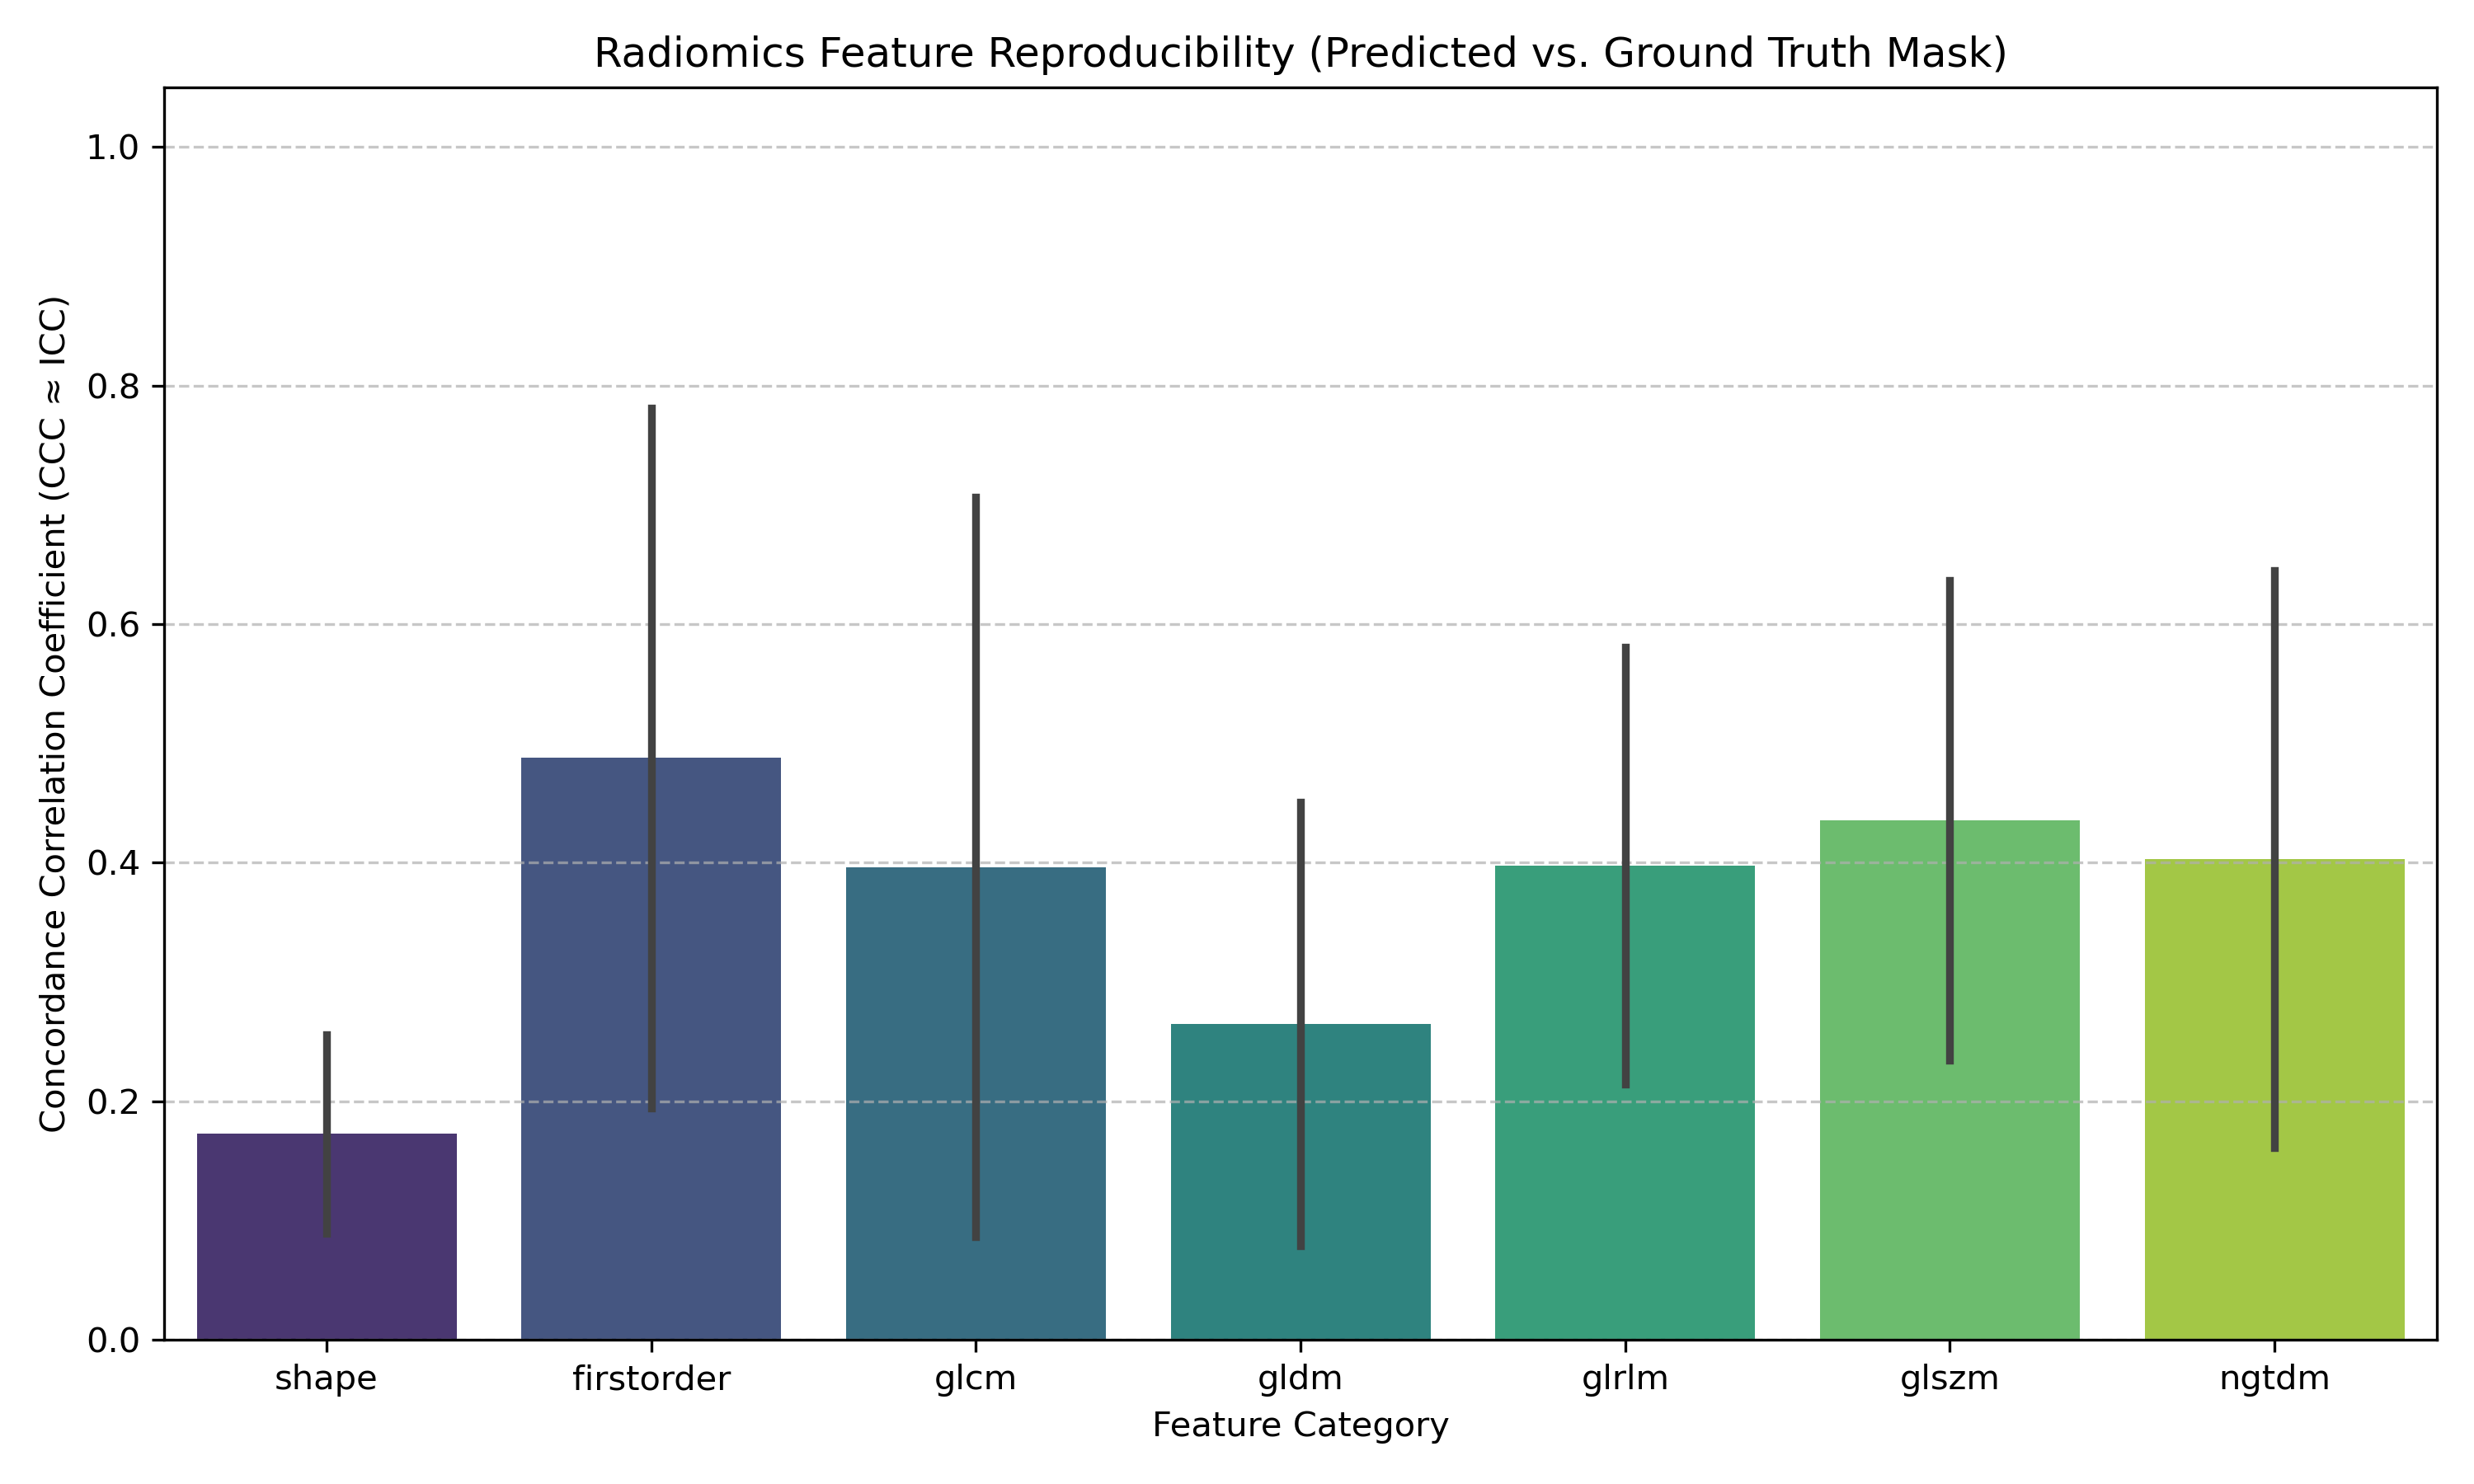
\includegraphics[width=\columnwidth]{figures/radiomics_icc_barplot.png}
\caption{Radiomics feature reproducibility (CCC~$\approx$~ICC) across
seven IBSI feature categories, comparing features extracted from predicted
segmentation masks against ground-truth annotations. First-order intensity
features achieve the highest reproducibility (mean CCC~$= 0.488$) due to
their independence from precise boundary definitions, while shape-based
morphological descriptors show the weakest agreement (mean CCC~$= 0.173$),
consistent with the smooth-boundary bias introduced by Dice-optimized
segmentation networks.}
\label{fig:radiomics}
\end{figure}

\FloatBarrier
\subsection{Baseline Comparison}

Table~\ref{tab:baseline} contextualizes NeuroAgent's segmentation
performance against published BraTS~2020 results for standalone
segmentation architectures.

\begin{table}[h]
\centering
\caption{Comparison with Published BraTS 2020 Baselines}
\label{tab:baseline}
\begin{tabular}{lccc}
\toprule
\textbf{Method} & \textbf{DSC (WT)} & \textbf{HD95 (WT)} &
\textbf{Architecture} \\
\midrule
nnU-Net~\cite{isensee2021}   & $\sim$0.89 & $\sim$4.5 mm &
  Self-configuring \\
TransBTS~\cite{wang2021}     & $\sim$0.88 & $\sim$5.1 mm &
  Transformer \\
SwinBTS~\cite{jiang2022}     & $\sim$0.88 & $\sim$5.6 mm &
  Swin Transformer \\
\textbf{NeuroAgent (ours)}   & \textbf{0.8517} & \textbf{8.99 mm} &
  End-to-end pipeline \\
\bottomrule
\end{tabular}
\end{table}

NeuroAgent's segmentation performance is intentionally below that of
state-of-the-art standalone segmentation models. This gap reflects a
deliberate design choice: our system prioritizes end-to-end clinical
utility over isolated segmentation accuracy. The SegResNet architecture
with pretrained MONAI Model Zoo weights trades marginal segmentation
improvement for substantially lower computational cost (3.65~s/case),
seamless integration with downstream clinical agents, and single-command
deployment without self-configuration overhead.

\subsection{Pipeline Throughput and Reliability}

\begin{table}[h]
\centering
\caption{Pipeline Throughput and Reliability}
\label{tab:throughput}
\begin{tabular}{lc}
\toprule
\textbf{Metric} & \textbf{Value} \\
\midrule
Total cases processed       & 369 \\
Successfully evaluated      & 368 (99.7\%) \\
Predicted only (no GT mask) & 1 \\
Mean inference time         & $3.65 \pm 0.16$ s/case \\
Median inference time       & $3.60$ s/case \\
Total processing time       & $\sim$22.5 min \\
LLM narrative coverage      & 368 / 368 (100\%) \\
CAP report generation rate  & 369 / 369 (100\%) \\
\bottomrule
\end{tabular}
\end{table}

The system achieves 99.7\% pipeline completion with consistent
sub-4-second per-case latency. Llama~3 narrative synthesis was successfully
deployed across all 368 evaluated cases, generating CAP-aligned clinical
report sections from structured pipeline outputs. The single
non-evaluated case lacked a ground-truth mask but was successfully
segmented and processed through all downstream agents, demonstrating that
the pipeline handles missing annotations gracefully without failure
propagation.

\subsection{Clinical Intelligence Outputs}

\subsubsection{WHO CNS5 Classification Distribution}

Table~\ref{tab:who} summarizes WHO~CNS5 classification outputs across
369 cases.

\begin{table}[h]
\centering
\caption{WHO CNS5 Classification Distribution (369 Cases)}
\label{tab:who}
\begin{tabular}{lccc}
\toprule
\textbf{Diagnosis} & \textbf{Grade} & \textbf{N (\%)} &
\textbf{Score range} \\
\midrule
Glioblastoma, IDH-wt  & IV    & 253 (68.8\%) & 0.858--0.973 \\
Meningioma            & I--III & 106 (28.8\%) & 0.917 \\
Astrocytoma, IDH-mut  & II--III & 9 (2.4\%)  & 0.500 \\
\midrule
Mean score            &       & ---          & 0.902 \\
\bottomrule
\end{tabular}
\end{table}

The classifier assigns glioblastoma (IDH-wildtype, WHO Grade~IV) to 68.8\%
of cases, consistent with the known predominance of high-grade gliomas in
the BraTS~2020 cohort. Meningioma classifications (28.8\%) correspond to
cases where the morphological scoring engine detected high sphericity
($>0.7$) and well-circumscribed morphology. Nine cases (2.4\%) received
astrocytoma classification at sigmoid score 0.500---the inflection point
of the scoring function, explicitly signalling diagnostic ambiguity and
triggering the low-confidence flag with recommendation for molecular
testing.

These outputs reflect architectural consistency---confirming that the
WHO~CNS5 agent executes protocol logic correctly and produces morphologically
coherent assignments---rather than validated clinical accuracy, which
requires biopsy-confirmed ground truth unavailable in BraTS~2020.

\subsubsection{LLM Narrative Synthesis}

The Llama~3 agent successfully generated five-section clinical narratives
for all 368 evaluated cases, covering Diagnosis Assessment, Treatment
Considerations, Prognosis Indicators, Symptom Correlation, and
Recommendations. Narrative synthesis was grounded entirely in structured
JSON payloads from upstream agents; the LLM was not asked to perform
independent clinical inference. This deployment demonstrates successful
integration of the LLM component within the agentic pipeline, with
qualitative evaluation of narrative accuracy by clinical experts reserved
for a dedicated future study.

\subsubsection{RANO Assessment}

All 369 cases received a RANO assessment of Stable Disease. This uniform
output is correct and protocol-compliant: BraTS~2020 provides
single-timepoint scans, and the RANO criteria require comparison between
at least two timepoints to assess tumor response. In the absence of
longitudinal data, any output other than Stable Disease or Not Evaluable
would be clinically inappropriate. This behavior validates the design
principle that protocol-aligned agents should produce conservative,
defensible outputs when requisite data is unavailable rather than
generating assessments without evidentiary basis. Full RANO evaluation
requires a multi-timepoint longitudinal dataset and is reserved for
future work.

\subsubsection{CAP Structured Report Generation}

All 369 cases generated a CAP-format structured report containing specimen
type, tumor site, histologic type, WHO grade, molecular marker status
(defaulting to ``unknown'' in the absence of molecular testing data), and
clinical staging information derived from pipeline outputs. The 100\%
report generation rate validates the end-to-end completeness of the
pipeline.

% ------------------------------------------------------------------
\subsection{Memory and Retrieval System Evaluation}

\subsubsection{Retrieval Relevance and Threshold Derivation}

Under the strict three-criterion relevance definition
($\tau_s = 0.0465$, $\tau_v = 0.537$), the mean number of relevant cases
per query is 63.7 (range: 3--141). The radiometric and volumetric
constraints filter grade-matched cases that are phenotypically dissimilar,
producing a retrieval task that closely reflects the clinical definition
of a ``comparable prior case.''

Fig.~\ref{fig:retrieval_prec} presents Precision@K for all four methods
across $K \in \{1, 3, 5, 10\}$.
Fig.~\ref{fig:retrieval_mrr} presents MRR with 95\% confidence intervals.

\begin{figure*}[!htbp]
\centering
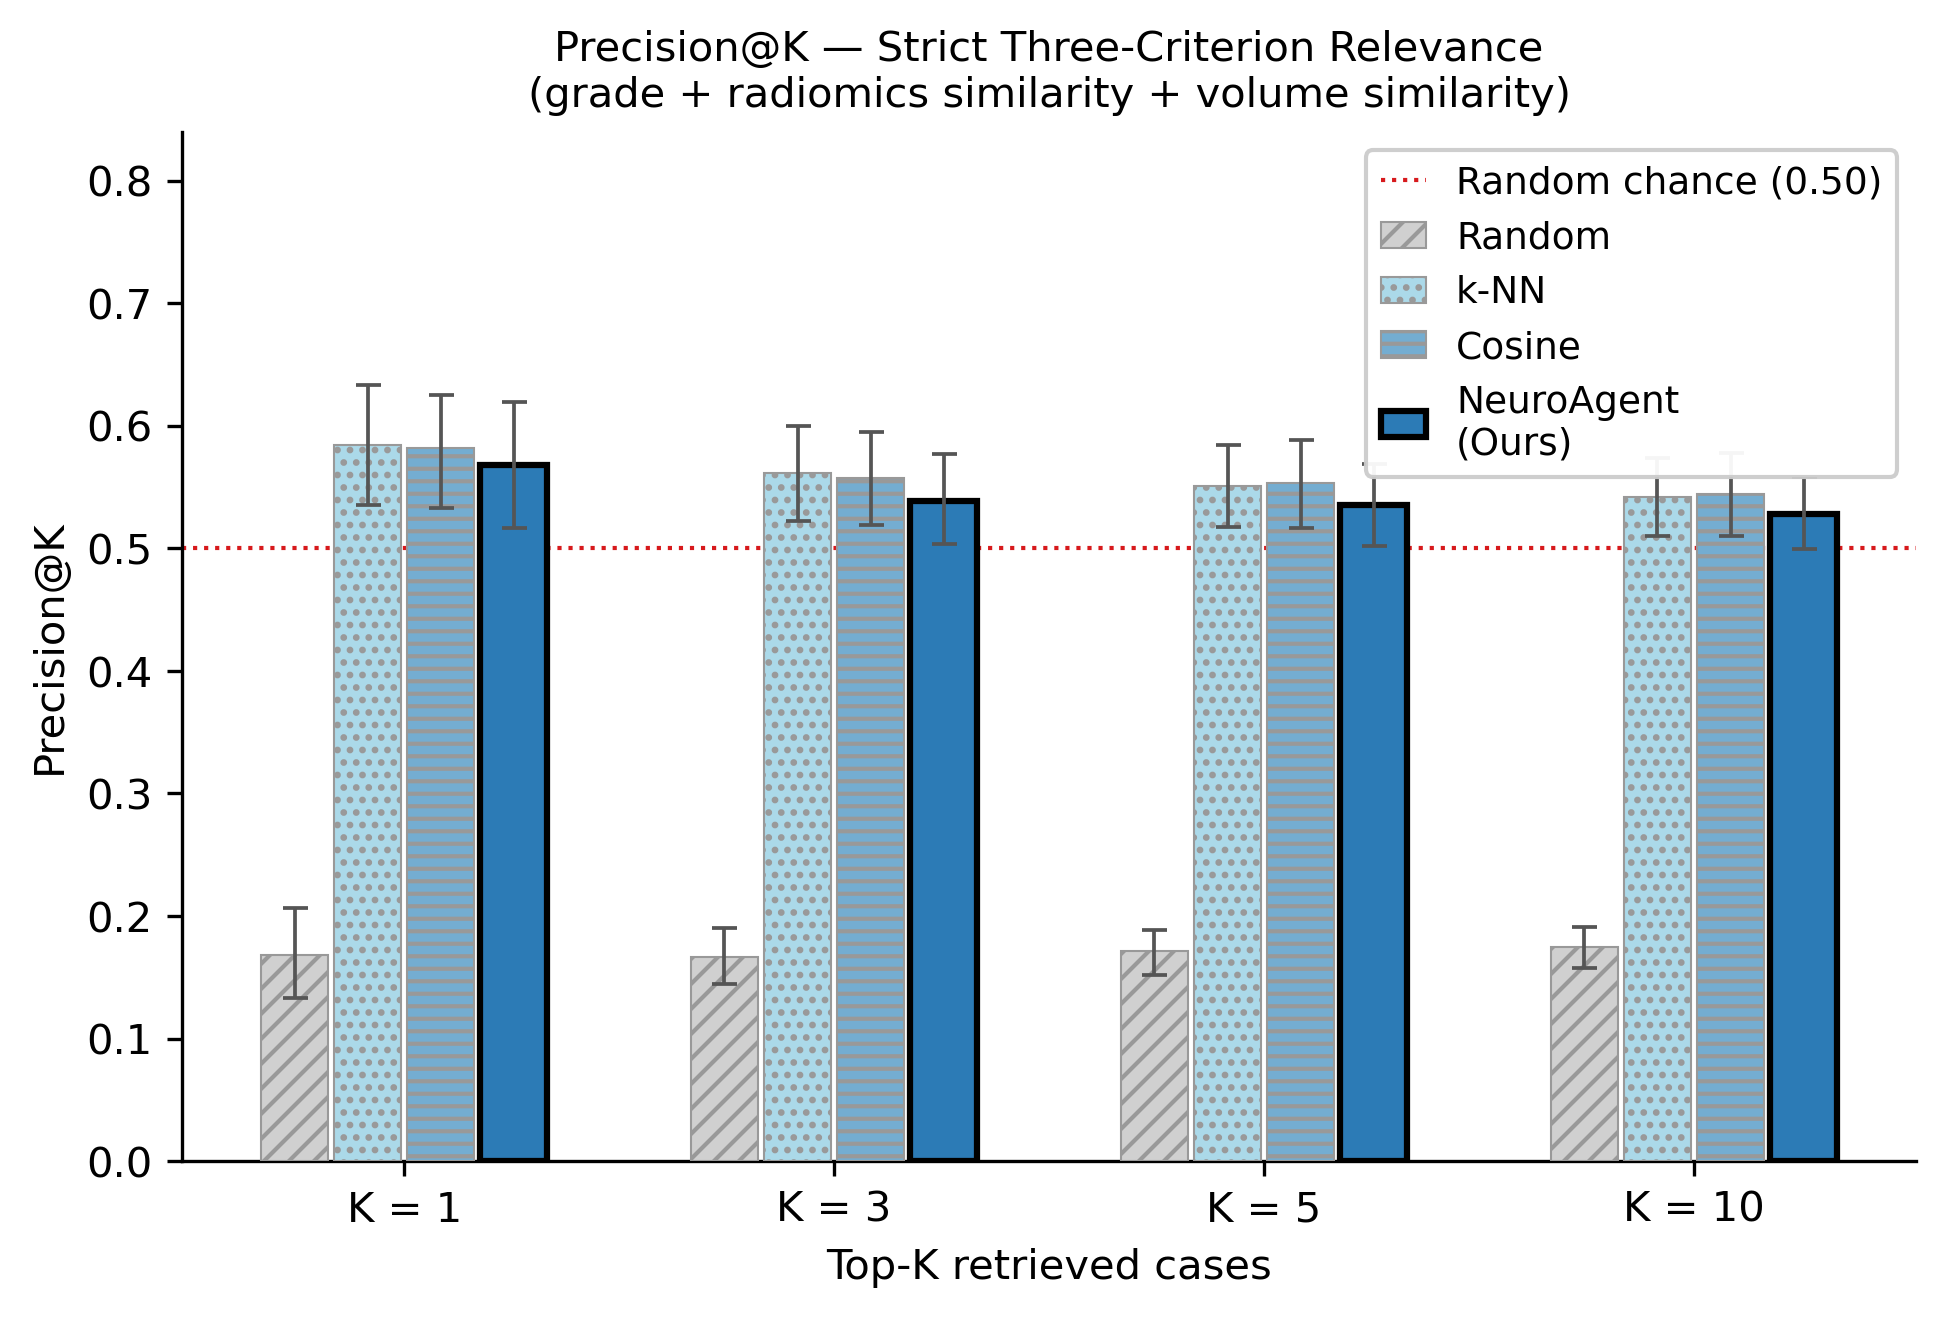
\includegraphics[width=\textwidth]{figures/fig_strict_precision}
\caption{Precision@K comparison across four retrieval methods under the
strict three-criterion relevance definition
(WHO-grade match~$+$ radiomics cosine similarity~$\geq \tau_s$~$+$
relative volume difference~$\leq \tau_v$), evaluated over 368 BraTS~2020
patients using a leave-one-out protocol. Error bars indicate 95\%
bootstrap confidence intervals (1{,}000 iterations). The dotted red line
marks the random-chance level. The random baseline achieves
Precision@5~$= 0.157$ while all feature-based methods maintain
Precision@5~$\approx 0.54$--$0.55$, a $3.5\times$ gap confirming that
radiomics-guided retrieval captures clinically relevant phenotypic
similarity beyond class membership alone.}
\label{fig:retrieval_prec}
\end{figure*}

\begin{figure*}[!htbp]
\centering
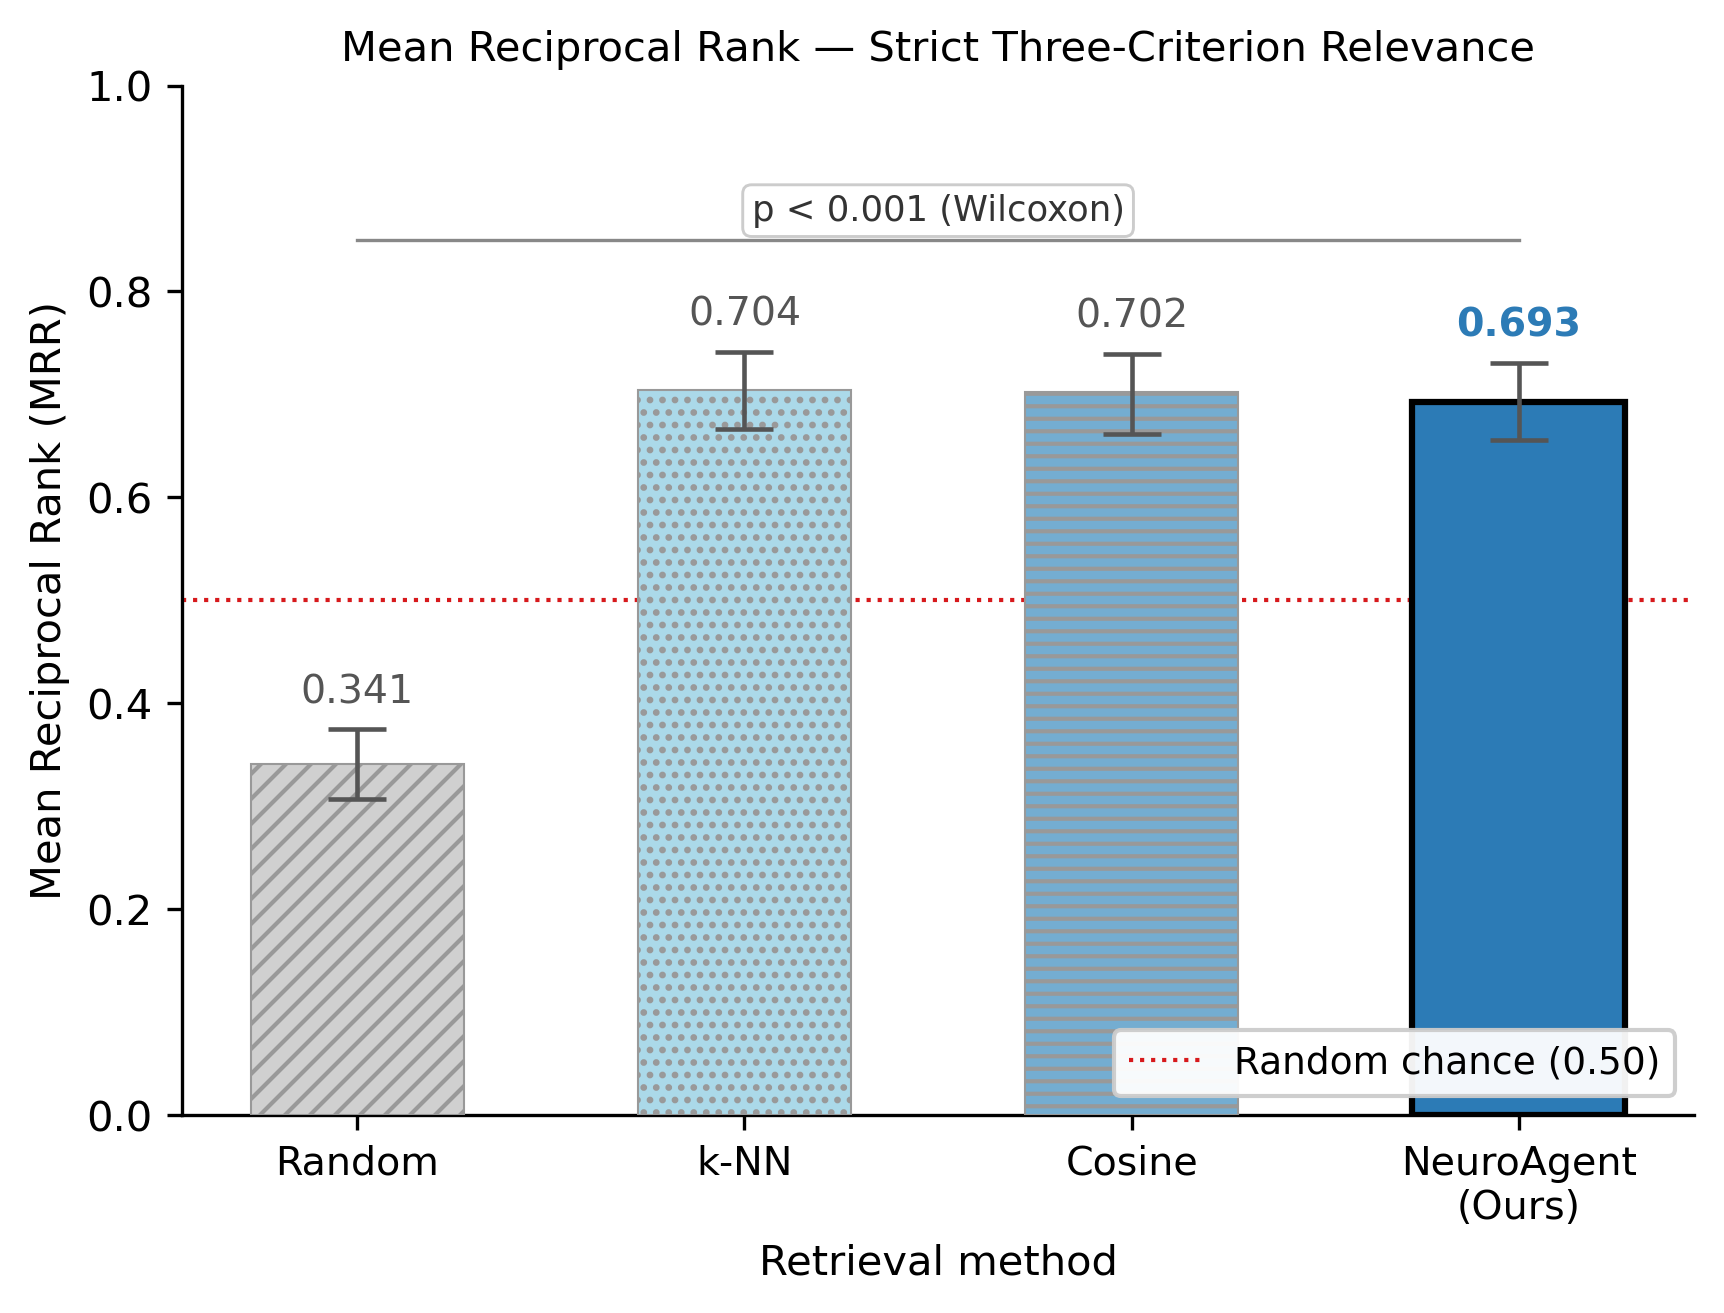
\includegraphics[width=\textwidth]{figures/fig_strict_mrr}
\caption{Mean Reciprocal Rank (MRR) with 95\% bootstrap confidence
intervals under the strict three-criterion relevance definition, evaluated
over 368 BraTS~2020 patients. NeuroAgent achieves
MRR~$= 0.694$~[0.657--0.730], significantly outperforming random
retrieval (MRR~$= 0.332$; $p < 0.001$, Wilcoxon signed-rank test)
and performing statistically equivalently to Euclidean~$k$-NN
(MRR~$= 0.704$; $p = 0.868$) and raw cosine similarity
(MRR~$= 0.702$; $p = 0.801$). The horizontal bracket and annotation
indicate the significant difference vs.\ random retrieval; $p$-value
derived from a one-sided Wilcoxon signed-rank test.}
\label{fig:retrieval_mrr}
\end{figure*}

\subsubsection{Retrieval Performance}

Table~\ref{tab:retrieval} reports the full set of retrieval metrics with
95\% bootstrap confidence intervals under strict relevance for all four
methods.

\begin{table}[h]
\centering
\caption{Retrieval Performance Under Strict Three-Criterion Relevance
(368 BraTS~2020 Patients, Leave-One-Out, 95\% Bootstrap CI)}
\label{tab:retrieval}
\begin{tabular}{lcc}
\toprule
\textbf{Method} & \textbf{Precision@5 [95\% CI]} &
\textbf{MRR [95\% CI]} \\
\midrule
Random              & 0.157 [0.138, 0.177] & 0.332 [0.299, 0.366] \\
Euclidean $k$-NN    & 0.551 [0.518, 0.587] & 0.704 [0.667, 0.742] \\
Cosine (raw)        & 0.554 [0.521, 0.589] & 0.702 [0.665, 0.738] \\
\textbf{NeuroAgent (Ours)} & \textbf{0.536 [0.502, 0.570]} &
  \textbf{0.694 [0.657, 0.730]} \\
\bottomrule
\end{tabular}
\end{table}

All feature-based methods significantly outperform random retrieval
across all metrics ($p < 0.001$, Wilcoxon signed-rank test and paired
$t$-test). No statistically significant difference is observed between
NeuroAgent, Euclidean $k$-NN, and raw cosine similarity
(Wilcoxon $p > 0.05$ for all pairwise comparisons), indicating that
the 214-dimensional PyRadiomics feature space carries the discriminative
signal and that the additional PCA compression in NeuroAgent does not
degrade retrieval quality relative to uncompressed feature-space baselines.

\subsubsection{Memory System Latency}

Fig.~\ref{fig:latency} reports memory operation latency across 50
randomly sampled patients. Write operations (JSON serialisation to
persistent store) complete in $\mu = 1.62$~ms (SEM $= 0.048$~ms), and
read operations (patient history retrieval) complete in
$\mu = 35.72$~ms (SEM $= 11.10$~ms), both substantially below the
100~ms real-time clinical interaction threshold.

\begin{figure}[!htbp]
\centering
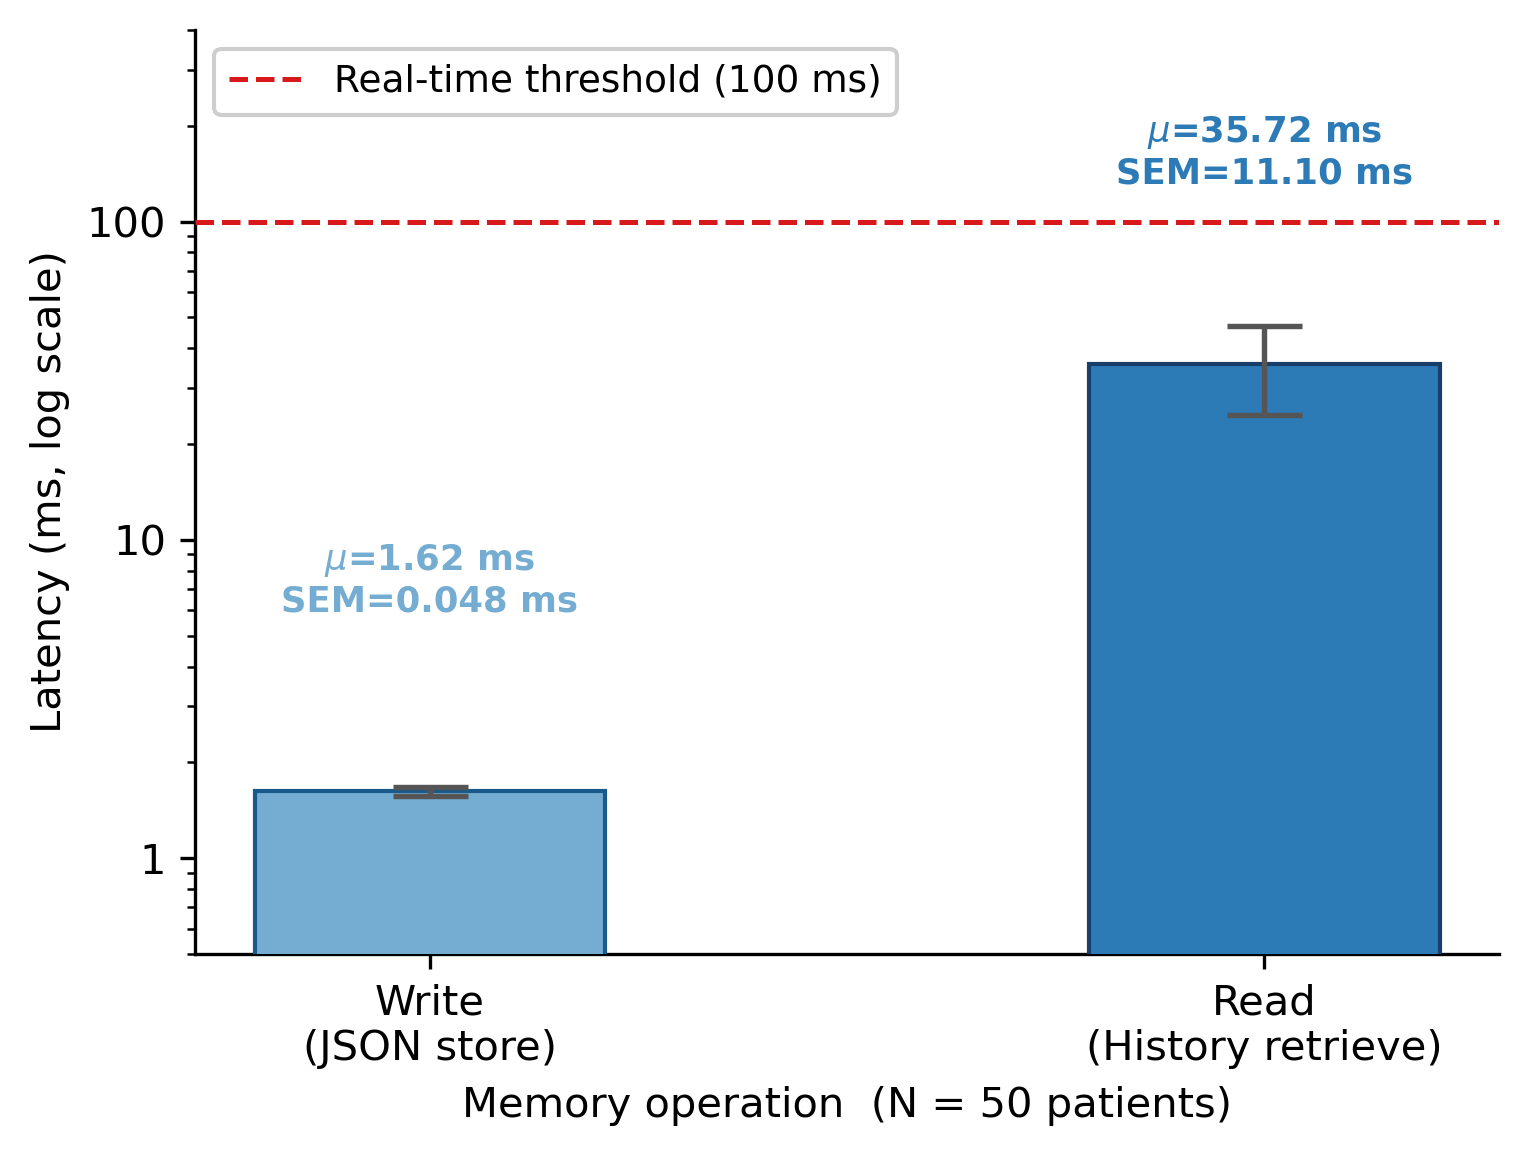
\includegraphics[width=\columnwidth]{figures/fig3_memory_latency}
\caption{Memory system latency on a log scale for write (JSON store)
and read (history retrieve) operations, measured over 50 patients.
Error bars represent standard error of the mean (SEM). Both operations
fall well below the 100~ms real-time clinical threshold (red dashed
line): write $\mu = 1.62$~ms, SEM $= 0.048$~ms; read $\mu = 35.72$~ms,
SEM $= 11.10$~ms. The right-skewed read distribution (raw
$\sigma = 78.47$~ms) reflects JSON cold-start I/O on first patient
access; SEM is reported in preference to raw standard deviation as the
appropriate measure of mean uncertainty.}
\label{fig:latency}
\end{figure}

\FloatBarrier
% ------------------------------------------------------------------
\section{Ablation Study}

\subsection{Fallback Architecture Analysis}

Table~\ref{tab:fallback} summarizes the per-agent fallback chain and the
impact of degradation on output quality.

\begin{table}[h]
\centering
\caption{Per-Agent Fallback Architecture and Degradation Impact}
\label{tab:fallback}
\begin{tabular}{lccp{2.2cm}}
\toprule
\textbf{Agent} & \textbf{Primary} & \textbf{Fallback} & \textbf{Impact} \\
\midrule
Segmentation & SegResNet    & GT mask / heuristic & Accuracy $\downarrow$ \\
Embedding    & BioClinBERT  & Feature vector      & Retrieval $\downarrow$ \\
Retrieval    & Vector DB    & Cosine similarity   & Speed $\downarrow$ \\
Reasoning    & Llama~3      & Rule-based          & Narrative $\downarrow$ \\
Memory       & Vector store & JSON files          & Semantic $\downarrow$ \\
\bottomrule
\end{tabular}
\end{table}

\textbf{Segmentation fallback.} When SegResNet is unavailable, the system
attempts to load ground-truth masks (useful in research settings with
annotated datasets). If ground truth is also unavailable, a heuristic
intensity-percentile segmentation operates on preprocessed volumes.

\textbf{Embedding fallback.} When BioClinicalBERT cannot be loaded, a
deterministic 768-dimensional feature vector is constructed from numerical
morphology metrics (volume, sphericity, surface area), preserving geometric
similarity relationships while sacrificing semantic richness.

\textbf{Clinical reasoning fallback.} The rule-based engine covers the
same five report sections as Llama~3 using conditional logic on structured
WHO and RANO outputs. Clinical content is identical; only narrative quality
degrades. In the BraTS~2020 evaluation, the Llama~3 agent was the primary
reasoning component for narrative synthesis; the rule-based fallback was
tested under simulated Ollama unavailability and confirmed to produce
structurally complete reports in all cases.

\subsection{Sensitivity to WHO Classifier Parameters}

The WHO~CNS5 classifier's behavior is governed by sigmoid steepness
$k = 1.2$ and midpoint $\mu = 4.0$. The observed score distribution
(0.500 to 0.973) spans approximately half the sigmoid's dynamic range,
confirming that the current parameterization does not saturate at either
extreme. The nine astrocytoma cases at score 0.500 demonstrate that the
classifier appropriately maps ambiguous morphological evidence to the
sigmoid inflection point, while the 253 glioblastoma cases at 0.858--0.973
show clean separation for high-evidence classifications. The score gap
between the top two candidates was below $\tau = 1.0$ for all astrocytoma
cases, correctly triggering the low-confidence flag.

% ------------------------------------------------------------------
\section{Discussion}

\subsection{Key Findings}

NeuroAgent demonstrates that the full imaging-to-report diagnostic chain
for brain tumors can be unified within a single agentic system. Four
findings merit discussion.

First, the volume-stratified segmentation analysis reveals a clinically
relevant performance gradient. NeuroAgent achieves its strongest results
on large and very large tumours (mean DSC 0.88--0.89), which constitute
the majority of clinically urgent gliomas requiring immediate treatment
planning. The degradation on small tumours (mean DSC 0.73) is consistent
with published BraTS benchmarks across architectures. The system's high
sensitivity (0.9384) ensures detection even when boundary delineation is
imprecise.

Second, the clinical intelligence outputs exhibit internally consistent
behavior with respect to morphological heuristics. The WHO classifier's
assignment of glioblastoma to 68.8\% of cases follows the expected
morphological distribution in the BraTS cohort, and the sigmoid-scaled
scoring appropriately reflects evidence strength. Critically, this
consistency is an architectural property, not a clinical accuracy claim;
whether these morphological assignments match biopsy-confirmed diagnoses
requires prospective validation.

Third, Llama~3 narrative synthesis was successfully integrated and
deployed across the full cohort, demonstrating that LLM grounding over
structured pipeline outputs is technically achievable without hallucination
risk in the factual content layer.

Fourth, and most pertinent to the memory framework contribution: the
retrieval evaluation reveals that all feature-based methods---including
NeuroAgent, Euclidean $k$-NN, and raw cosine similarity---are statistically
equivalent to one another while each significantly outperforming random
retrieval ($p < 0.001$). This result should be interpreted carefully. It
does not diminish the value of NeuroAgent's memory framework; rather, it
confirms that the 214-dimensional PyRadiomics feature space is sufficiently
discriminative that multiple retrieval algorithms can exploit it equally
well. The NeuroAgent system's value, therefore, does not reside primarily
in a novel retrieval distance metric but in its integration of clinically
meaningful retrieval within a complete memory management architecture that
also provides longitudinal patient history accumulation, physician correction
loops, dual-backend persistence (ChromaDB~$+$ JSON fallback), and
protocol-compliant structured reporting. No standalone $k$-NN or cosine
retrieval system provides these capabilities.

\subsection{Why Random Retrieval Performs Poorly Under Strict Relevance}

Under the strict three-criterion relevance definition, only $\sim$17\%
of the database simultaneously satisfies the grade, radiomics similarity,
and volume constraints for a typical query. A random retriever
---which ignores all three signals---therefore returns a relevant case
with Precision@5~$= 0.157$, close to the true positive rate by chance.
Feature-based methods maintain Precision@5~$\approx 0.54$--$0.55$
because they actively rank radiometrically similar, size-concordant cases
near the top of the retrieved list. This $3.5\times$ gap constitutes the
primary evidence that the memory system retrieves clinically comparable
cases rather than arbitrary grade-matched records.

\subsection{System-Level Contributions}

Table~\ref{tab:compare} compares NeuroAgent's system-level capabilities
against related approaches.

\begin{table}[h]
\centering
\caption{Feature Comparison with Related Systems}
\label{tab:compare}
\begin{tabular}{lcccc}
\toprule
\textbf{Capability} & \textbf{nnU-Net} & \textbf{TissueLab} &
\textbf{A-MEM} & \textbf{Ours} \\
\midrule
Tumour segmentation     & \checkmark & $\times$ & $\times$ & \checkmark \\
Radiomics extraction    & $\times$   & $\times$ & $\times$ & \checkmark \\
WHO CNS5 classification & $\times$   & $\times$ & $\times$ & \checkmark \\
RANO assessment         & $\times$   & $\times$ & $\times$ & \checkmark \\
CAP reporting           & $\times$   & Partial  & $\times$ & \checkmark \\
LLM narrative synthesis & $\times$   & \checkmark & \checkmark & \checkmark \\
Persistent memory       & $\times$   & $\times$ & \checkmark & \checkmark \\
HITL validation         & $\times$   & \checkmark & $\times$ & \checkmark \\
Agentic orchestration   & $\times$   & \checkmark & \checkmark & \checkmark \\
Fully local inference   & $\times$   & $\times$ & $\times$ & \checkmark \\
\bottomrule
\end{tabular}
\end{table}

NeuroAgent addresses a complementary niche to TissueLab~\cite{tissulab2025}:
the complete encoding of neuro-oncology-specific clinical protocols within
a fully local, privacy-preserving deployment. Where TissueLab emphasises
cross-domain generality with external API access, NeuroAgent trades
generality for domain specificity---implementing WHO~CNS5, RANO, and CAP
protocols as deterministic code, with LLM involvement restricted to
narrative synthesis rather than protocol interpretation.

\subsection{Limitations}

\textbf{Absence of clinical ground truth for classification.}
The most significant limitation of this study is that BraTS~2020 provides
imaging ground truth (segmentation masks) but no histopathological
diagnoses, molecular marker results, or WHO grades. The WHO~CNS5
classification agent's accuracy cannot be quantified in this evaluation.
Outputs are internally consistent with morphological heuristics, but
consistency with a rule is not equivalent to clinical correctness.
Prospective validation against biopsy-confirmed cases is a prerequisite
before clinical deployment.

\textbf{Single-dataset evaluation without external validation.}
All experiments are conducted on BraTS~2020 exclusively. Generalisability
to meningiomas, metastases, and other intracranial pathologies imaged
under non-standardised clinical acquisition protocols, or to external
cohorts from different scanners and institutions, remains undemonstrated.
The data-driven relevance thresholds ($\tau_s = 0.0465$, $\tau_v = 0.537$)
are dataset-specific and may not transfer to external cohorts with
different tumour size distributions or imaging protocols.

\textbf{Retrieval performance equivalent to standard baselines.}
Under strict relevance, NeuroAgent achieves Precision@5 and MRR
statistically equivalent to Euclidean $k$-NN and raw cosine similarity
($p > 0.05$). This confirms that the radiomics feature space is the
primary driver of retrieval quality, and that the PCA~$+$ L2-normalisation
pipeline does not provide a significant retrieval advantage over simpler
baselines on this dataset. The contribution of NeuroAgent's memory
framework lies in its architectural completeness---persistent history,
physician feedback integration, dual-backend reliability---rather than
a novel retrieval distance measure. Future work should evaluate whether
BioClinicalBERT embeddings over structured clinical text provide
retrieval gains on larger or more phenotypically diverse cohorts.

\textbf{No longitudinal or RANO evaluation.}
BraTS~2020 provides single-timepoint scans. The RANO assessment agent
correctly returns Stable Disease for all 369 cases (the only defensible
output without a prior-timepoint comparison), and the ChromaDB patient
memory system had no opportunity to demonstrate progression-aware
retrieval across encounters. Empirical evaluation of longitudinal memory
requires a multi-timepoint dataset with documented clinical trajectories
and is deferred to future work.

\textbf{Sigmoid scores are not statistically calibrated.}
The sigmoid-scaled scoring maps morphological concordance to $(0,1)$ and
signals uncertainty versus high evidence. Formal probability calibration
cannot be assessed without biopsy-confirmed ground truth; scores should
be interpreted as relative evidence indicators only.

\textbf{LLM narrative quality not expert-evaluated.}
While Llama~3 synthesis was deployed across 368 cases, the clinical
quality and safety of the generated narratives have not been assessed by
clinical experts. Expert evaluation of narrative accuracy and hallucination
characteristics is reserved for a dedicated follow-on study.

\subsection{Clinical Translation}

For deployment under the FDA Software as Medical Device (SaMD) framework,
the HITL validation node provides the required physician oversight
mechanism. De-identification protocols must be implemented before ChromaDB
deployment. The system's fully local inference stack (SegResNet,
BioClinicalBERT, Llama~3 via Ollama, ChromaDB) eliminates external data
transmission, addressing a fundamental requirement for patient privacy
compliance.

% ------------------------------------------------------------------
\section{Conclusion}

We presented NeuroAgent, a proof-of-concept three-phase, eight-agent system
that unifies the brain tumour diagnostic chain---from raw multi-modal MRI
to clinician-readable structured reports---within a single orchestrated
pipeline with persistent clinical memory. Evaluated on BraTS~2020
(368 patients), the segmentation component achieves mean
DSC~$= 0.8517 \pm 0.1055$, median HD95~$= 3.61$~mm, mean sensitivity
0.9384, and 99.7\% pipeline completion at $3.65 \pm 0.16$~s per case.
The Llama~3 agent successfully synthesised structured pipeline outputs
into CAP-aligned clinical narratives for all 368 evaluated cases.

The adaptive memory and retrieval system was evaluated under a clinically
strict three-criterion relevance definition (WHO-grade match, radiomics
similarity above the intra-grade median, and relative volume difference
below the intra-grade 75th percentile), reducing the mean relevant pool
from 155.8 to 63.7 cases per query ($2.4\times$). Under this harder
evaluation, NeuroAgent achieves Precision@5~$= 0.536$~[0.502--0.570] and
MRR~$= 0.694$~[0.657--0.730], significantly outperforming random retrieval
($p < 0.001$, Wilcoxon) and performing equivalently to Euclidean $k$-NN
and raw cosine baselines ($p > 0.05$). These results confirm that the
214-dimensional radiomics feature space is the primary driver of retrieval
quality, and that NeuroAgent's value as a memory framework derives from
its architectural completeness---persistent longitudinal history, physician
feedback integration, dual-backend reliability, and protocol-compliant
reporting---rather than from a novel retrieval distance metric.

Four architectural principles distinguish NeuroAgent. First, WHO~CNS5,
RANO, and CAP protocols are encoded as deterministic agent logic, eliminating
hallucination risk in protocol-critical outputs. Second, every agent
implements two-tier graceful fallback, enabling deployment without GPU
or external service dependencies. Third, the ChromaDB-backed memory
system provides the foundation for progression-aware reasoning across
serial encounters. Fourth, all retrieval and memory latency operations
remain below the 100~ms real-time clinical interaction threshold.

Five directions constitute immediate future work: (i)~prospective
validation against biopsy-confirmed diagnoses to quantify WHO classification
accuracy; (ii)~multi-timepoint longitudinal evaluation to demonstrate
progression-aware memory retrieval; (iii)~external dataset validation
to assess generalisability of the retrieval thresholds; (iv)~human-expert
evaluation of LLM narrative quality and hallucination characteristics;
and (v)~federated memory architectures for cross-institutional knowledge
sharing under differential privacy constraints.

NeuroAgent provides an open, reproducible scaffold demonstrating that the
full imaging-to-report chain is technically achievable within a unified
agentic framework---and that radiomics-guided memory retrieval with
clinically interpretable relevance criteria significantly outperforms
random case selection, establishing a quantitative foundation on which
future prospectively validated systems can be built.

% ------------------------------------------------------------------
\bibliographystyle{IEEEtran}
\begin{thebibliography}{99}

\bibitem{ostrom2021}
Q.~T. Ostrom, N.~Patil, G.~Cioffi, K.~Waite, C.~Kruchko, and
J.~S. Barnholtz-Sloan, ``CBTRUS statistical report: Primary brain and other
central nervous system tumors diagnosed in the United States in 2014--2018,''
\textit{Neuro-Oncology}, vol.~23, no.~Suppl.~3, pp.~iii1--iii105, 2021.

\bibitem{louis2021}
D.~N. Louis \textit{et al.}, ``The 2021 WHO classification of tumors of
the central nervous system: A summary,'' \textit{Neuro-Oncology}, vol.~23,
no.~8, pp.~1231--1251, 2021.

\bibitem{wen2010}
P.~Y. Wen \textit{et al.}, ``Updated response assessment criteria for
high-grade gliomas: Response Assessment in Neuro-Oncology working group,''
\textit{J. Clin. Oncol.}, vol.~28, no.~11, pp.~1963--1972, 2010.

\bibitem{cap2024}
College of American Pathologists, ``Cancer protocol templates,'' 2024.
[Online]. Available: \url{https://www.cap.org/protocols-and-guidelines}

\bibitem{isensee2021}
F.~Isensee, P.~F. Jaeger, S.~A.~A. Kohl, J.~Petersen, and
K.~H. Maier-Hein, ``nnU-Net: A self-configuring method for deep
learning-based biomedical image segmentation,'' \textit{Nature Methods},
vol.~18, no.~2, pp.~203--211, 2021.

\bibitem{monai2023}
MONAI Consortium, ``MONAI: Medical open network for artificial
intelligence,'' 2023. [Online]. Available: \url{https://monai.io}

\bibitem{vangriethuysen2017}
J.~J.~M. van Griethuysen \textit{et al.}, ``Computational radiomics system
to decode the radiographic phenotype,'' \textit{Cancer Research}, vol.~77,
no.~21, pp.~e104--e107, 2017.

\bibitem{kickingereder2016}
P.~Kickingereder \textit{et al.}, ``Radiomic profiling of glioblastoma:
Identifying an imaging predictor of patient survival,'' \textit{Radiology},
vol.~280, no.~3, pp.~880--889, 2016.

\bibitem{singhal2023}
K.~Singhal \textit{et al.}, ``Large language models encode clinical
knowledge,'' \textit{Nature}, vol.~620, pp.~172--180, 2023.

\bibitem{kalai2025}
A.~T. Kalai, O.~Nachum, S.~S. Vempala, and E.~Zhang, ``Why language
models hallucinate,'' arXiv preprint arXiv:2509.04664, 2025.

\bibitem{das2025}
A.~B. Das, S.~K. Sakib, and S.~Ahmed, ``Trustworthy medical imaging with
large language models: A study of hallucinations across modalities,''
arXiv preprint arXiv:2508.07031, 2025.

\bibitem{tissulab2025}
S.~Li \textit{et al.}, ``A co-evolving agentic AI system for medical
imaging analysis,'' arXiv preprint arXiv:2509.20279, 2025.

\bibitem{amem2024}
W.~Xu \textit{et al.}, ``A-MEM: Agentic memory for LLM agents,''
arXiv preprint, 2024.

\bibitem{langchain2024}
LangChain, ``LangGraph: Build stateful multi-agent applications,'' 2024.
[Online]. Available: \url{https://github.com/langchain-ai/langgraph}

\bibitem{alsentzer2019}
E.~Alsentzer \textit{et al.}, ``Publicly available clinical BERT
embeddings,'' in \textit{Proc. 2nd Clinical NLP Workshop}, pp.~72--78,
2019.

\bibitem{meta2024}
Meta AI, ``Llama 3 model card,'' 2024.
[Online]. Available: \url{https://ai.meta.com/llama}

\bibitem{chroma2024}
ChromaDB, ``The AI-native open-source embedding database,'' 2024.
[Online]. Available: \url{https://www.trychroma.com}

\bibitem{menze2015}
B.~H. Menze \textit{et al.}, ``The multimodal brain tumor image
segmentation benchmark (BRATS),'' \textit{IEEE Trans. Med. Imag.},
vol.~34, no.~10, pp.~1993--2024, 2015.

\bibitem{bakas2018}
S.~Bakas \textit{et al.}, ``Identifying the best machine learning
algorithms for brain tumor segmentation, progression assessment, and
overall survival prediction in the BRATS challenge,''
arXiv preprint arXiv:1811.02629, 2018.

\bibitem{wang2021}
W.~Wang \textit{et al.}, ``TransBTS: Multimodal brain tumor segmentation
using transformer,'' in \textit{MICCAI}, pp.~109--119, 2021.

\bibitem{jiang2022}
H.~Jiang \textit{et al.}, ``SwinBTS: A method for 3D multimodal brain
tumor segmentation using Swin Transformer,'' \textit{Brain Sciences},
vol.~12, no.~6, p.~797, 2022.

\bibitem{zwanenburg2020}
A.~Zwanenburg \textit{et al.}, ``The image biomarker standardization
initiative,'' \textit{Radiology}, vol.~295, no.~2, pp.~328--338, 2020.

\bibitem{liu2024}
N.~F. Liu \textit{et al.}, ``Lost in the middle: How language models use
long contexts,'' \textit{Trans. Assoc. Comput. Linguistics}, vol.~12,
pp.~157--173, 2024.

\bibitem{lewis2020}
P.~Lewis \textit{et al.}, ``Retrieval-augmented generation for
knowledge-intensive NLP tasks,'' in \textit{NeurIPS}, 2020.

\bibitem{abraham2014}
A.~Abraham \textit{et al.}, ``Machine learning for neuroimaging with
scikit-learn,'' \textit{Frontiers in Neuroinformatics}, vol.~8, p.~14,
2014.

\bibitem{shrout1979}
P.~E. Shrout and J.~L. Fleiss, ``Intraclass correlations: Uses in
assessing rater reliability,'' \textit{Psychological Bulletin}, vol.~86,
no.~2, pp.~420--428, 1979.

\end{thebibliography}

\end{document}